\documentclass[fontset=windows]{article}
\usepackage{ctex}
\usepackage[margin=1in]{geometry}%设置边距,符合Word设定
\usepackage{listings}
\usepackage{color}
\usepackage[dvipsnames]{xcolor}
\usepackage{setspace}
\usepackage{booktabs,multirow}
\usepackage{float}
\usepackage{subfigure}
\usepackage[graphicx]{realboxes}
\usepackage[hidelinks]{hyperref}
\usepackage{titling}

\renewcommand\maketitlehooka{\null\mbox{}\vfill}
\renewcommand\maketitlehookd{\vfill\null}


\lstset{
    columns=fullflexible,
    language=bash,
    basicstyle=\ttfamily,
    showstringspaces=false,
    commentstyle=\color{BlueGreen},
    keywordstyle=\color{blue},
    breaklines=true, 
    frame=tb
}

\def\lstlistingname{代码}

\AtBeginDocument{\counterwithin{lstlisting}{section}}

\renewcommand\thefigure{\arabic{section}-\arabic{figure}}

\newcommand{\upcite}[1]{\textsuperscript{\cite{#1}}}

\title{\heiti\zihao{2} 操作系统课程设计实验报告}

\author{\fangsong 黄毅成}
\date{2024.7.16}

\begin{document}

\begin{titlingpage}
    \maketitle
\end{titlingpage}

\begin{center}
    \pagenumbering{Roman}
    \tableofcontents
\end{center}
\subsubsection*{实验代码仓库}
\textbf{\href{https://github.com/saikewei/xv-6-Lab}{https://github.com/saikewei/xv-6-Lab}}

\newpage
\pagenumbering{arabic}



\section{Lab: Xv6 and Unix utilities}
\subsection{实验目的}

本实验旨在熟悉xv6操作系统及其系统调用。通过本次实验,我将学习如何在xv6环境中设置并运行操作系统,理解并实现基本的UNIX实用程序。这包括启动xv6、获取并管理源代码、编译和运行操作系统、以及实现和测试具体的系统调用和应用程序。本实验将帮助深入理解操作系统的运行机制和开发流程,为后续更复杂的操作系统编程打下坚实基础。

具体将实现以下程序:
\begin{itemize}
    \item sleep程序:编写一个xv6版本的sleep程序,使其根据用户指定的ticks暂停。
    \item pingpong程序:编写一个使用管道和fork系统调用在父子进程间传递字节的程序。
    \item primes程序:编写一个基于管道的并发素数筛选程序,将数值在进程间传递并筛选素数。
    \item find程序:编写一个简化版的find程序,遍历目录树查找特定文件名。
    \item xargs程序:编写一个简化版的xargs程序,从标准输入读取行并为每行运行一个命令。
\end{itemize}

在实现和测试这些系统调用的过程中,我们将深入理解操作系统的内部机制,并掌握如何在用户程序中调用这些功能。
\subsection{实验步骤}
\subsubsection{运行xv6}
\begin{enumerate}
    \item 利用以下指令获取Lab xv6源代码,查看util分支。
          \begin{lstlisting}
    $ git clone git://g.csail.mit.edu/xv6-labs-2021
    $ cd xv6-labs-2021
    $ git checkout util
        \end{lstlisting}
    \item 输入make qemu命令构建并运行xv6。
          \begin{lstlisting}
    $ make qemu
    
    ...

    xv6 kernel is booting

    hart 2 starting
    hart 1 starting
    init: starting sh
        \end{lstlisting}
\end{enumerate}

\subsubsection{实现sleep}

\begin{enumerate}
    \item 根据题目提示,可以实现如下代码:
          \begin{lstlisting}[language=c, title=sleep.c]
    #include "kernel/types.h"   // 包含内核类型定义
    #include "user/user.h"      // 包含用户模式下的库函数

    int main(int argc, char *argv[])
    {
        // 检查命令行参数是否等于2,即程序名和等待时间参数
        if (argc != 2)
        {
            fprintf(2, "Error: Parameters Error\n"); // 打印错误信息
            exit(1); // 退出程序,返回状态码1
        }

        sleep(atoi(argv[1])); // 调用 sleep 函数,等待指定的秒数

        exit(0); // 程序正常退出,返回状态码0
    }
        \end{lstlisting}
    \item 在 Makefile 文件中的UPROGS加上\$U/\_sleep\textbackslash 后利用make qemu命令编译启动xv6操作系统;
    \item 在xv6命令行中运行sleep,程序将暂停执行一段指定的时间:
          \begin{lstlisting}
    $ sleep 10
        \end{lstlisting}
\end{enumerate}

\subsubsection{实现pingpong}

\begin{enumerate}
    \item 首先创建两条管道和用于储存数据的缓冲区。
          \begin{lstlisting}[language=c,title=初始化管道和缓冲区]
    int fd1[2];
    int fd2[2];

    pipe(fd1);
    pipe(fd2);

    char buffer[16];
            \end{lstlisting}
    \item 利用fork()创建子进程。
          \begin{lstlisting}[language=c,title=fork()函数]
    if (fork() != 0)
    {
        // 父线程执行的代码...
    }
    else
    {
        // 子线程执行的代码...
    }
            \end{lstlisting}
    \item 在父进程中发送“ping”并接收“pong”。
          \begin{lstlisting}[language=c, title=父进程]
    // 父线程执行的代码
    write(fd1[1], "ping", strlen("ping"));
    read(fd2[0], buffer, 4);
    printf("%d: received %s\n", getpid(), buffer);
    \end{lstlisting}
    \item 在子进程中发送“pong”并接收“ping”。
          \begin{lstlisting}[language=c, title=子进程]
    // 子线程执行的代码
    read(fd1[0], buffer, 4);
    printf("%d: received %s\n", getpid(), buffer);
    write(fd2[1], "pong", strlen("pong"));
    \end{lstlisting}
    \item 把程序写在pingpong.c中,用同样的方法在xv6中运行程序,可以观察到父子进程分别输出的结果。
          \begin{lstlisting}
    $ pingpong
    5: received ping
    4: received pong
    \end{lstlisting}
\end{enumerate}

\subsubsection{实现 prime}
\begin{enumerate}
    \begin{figure}[h]
        \centering
        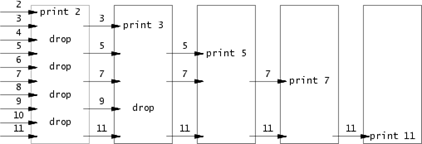
\includegraphics[width=\linewidth]{pics/图片1.png}
        \caption{primes程序原理}
        \label{fig:primes}
    \end{figure}
    \item 首先了解程序的原理。原理示意见图\ref{fig:primes}。程序通过递归创建进程和使用管道通信的方式,逐步筛选出素数。每个进程从管道中读取数值,将第一个数识别为素数,并过滤掉其倍数,然后将剩余的数传递给下一个进程继续处理,从而并发地筛选出所有素数。
    \item 把输出质数,创建子进程并向其传送数据的过程整合为一个递归函数。要注意文件描述符的回收,防止资源超限。
          \begin{lstlisting}[language=c, title=new\_prime\_proc函数的实现]
    void new_prime_proc(int *old_pipe)
    {
        close(old_pipe[1]); // 关闭旧管道的写端

        int first_num;
        // 从旧管道中读取第一个数,如果读取失败则退出
        if (!read(old_pipe[0], &first_num, sizeof(first_num)))
        {
            close(old_pipe[0]); // 关闭旧管道的读端
            exit(0);            // 退出进程
        }

        fprintf(1, "prime %d\n", first_num); // 打印第一个数,即当前的素数

        int new_pipe[2];
        pipe(new_pipe); // 创建新管道

        int p_id = fork(); // 创建子进程
        if (p_id == 0)
            new_prime_proc(new_pipe); // 子进程递归调用处理新管道
        else
        {
            int t;
            // 在父进程中,从旧管道中读取数,如果不是first_num的倍数则写入新管道
            while (read(old_pipe[0], &t, sizeof(t)))
            {
                if (t % first_num != 0)
                {
                    write(new_pipe[1], &t, sizeof(t));
                }
            }

            close(old_pipe[0]); // 关闭旧管道的读端
            close(new_pipe[0]); // 关闭新管道的读端
            close(new_pipe[1]); // 关闭新管道的写端

            wait((int *)0); // 等待子进程结束
        }
    }
    \end{lstlisting}
    \item 在主函数中将2~35写入管道,调用递归函数。
          \begin{lstlisting}[language=c, title=main()函数的实现]
    int main()
    {
        int p[2];
        pipe(p); // 创建管道
        int i;
        // 向管道中写入从2到35的所有数
        for (i = 2; i <= 35; i++)
            write(p[1], &i, sizeof(i));
        new_prime_proc(p); // 调用处理函数处理管道中的数
    
        exit(0); // 退出程序
    }
    \end{lstlisting}
    \item 把程序写在primes.c中,运行程序得到结果。
          \begin{lstlisting}
    $ primes
    prime 2
    prime 3
    ...
    prime 31
    \end{lstlisting}
\end{enumerate}

\subsubsection{实现 find}

\begin{enumerate}
    \item 首先,仿照ls.c实现一个辅助函数char*fmtname(char *path),把路径末尾的文件名提取出来,实现过程略。
    \item 利用深度优先搜索的思想,实现一个find函数递归寻找文件。
          \begin{lstlisting}[language=c, title=find函数的实现]
    void find(char *path, char *target)
    {
        char buf[512], *p;
        int fd;
        struct dirent de;
        struct stat st;

        // 打开指定路径的文件或目录
        if ((fd = open(path, 0)) < 0)
        {
            fprintf(2, "find: cannot open %s\n", path);
            return;
        }

        // 获取文件或目录的状态信息
        if (fstat(fd, &st) < 0)
        {
            fprintf(2, "find1: cannot stat %s\n", path); 
            close(fd);
            return;
        }

        // 根据文件或目录的类型进行处理
        switch (st.type)
        {
        case T_FILE:
            // 如果是文件,比较文件名是否与目标名称相同
            if (strcmp(target, path2name(path)) == 0)
            {
                printf("%s\n", path); // 输出文件路径
            }

            break;
        case T_DIR:
            // 如果是目录,检查路径长度是否超出缓冲区范围
            if (strlen(path) + 1 + DIRSIZ + 1 > sizeof buf)
            {
                printf("find: path too long\n"); // 输出错误信息,路径过长
                break;
            }
            strcpy(buf, path); // 将路径复制到缓冲区
            p = buf + strlen(buf);
            *p++ = '/';

            // 遍历目录中的每个文件或子目录
            while (read(fd, &de, sizeof(de)) == sizeof(de))
            {
                if (de.inum == 0)
                    continue; // 跳过空目录项

                memmove(p, de.name, DIRSIZ); // 将文件或目录名复制到缓冲区末尾
                p[DIRSIZ] = 0;               // 添加字符串结束符

                // 获取文件或目录的状态信息
                if (stat(buf, &st) < 0)
                {
                    // 输出错误信息,无法获取文件或目录的状态信息
                    printf("find2: cannot stat %s\n", buf); 
                    continue;
                }

                // 排除当前目录和上级目录的特殊情况
                if (strlen(de.name) == 1 && de.name[0] == '.')
                    continue;
                if (strlen(de.name) == 2 
                && de.name[0] == '.' 
                && de.name[1] == '.')
                    continue;
                find(buf, target); // 递归调用查找函数,继续查找子目录
            }
            break;
        }

        close(fd); // 关闭文件或目录
    }
    \end{lstlisting}
    \item 在主函数中调用find函数。
    \item 将程序写在find.c中,运行程序得到结果。
          \begin{lstlisting}
    $ find . b
    ./a/b
    ./b
    \end{lstlisting}
\end{enumerate}

\subsubsection{实现 xargs}
\begin{enumerate}
    \item 首先初始化一些变量。
          \begin{lstlisting}[language=c, title=初始化]
    int i;
    int arg_count = 0;  // 参数数量计数器
    char *args[MAXARG]; // 参数数组,最大长度为MAXARG
    int initial_arg_count = arg_count; // 存储初始参数数量的位置
    
    int line_index = 0; // 当前行的索引
    char input_char;                   // 用于读取字符
    char *current_line;                // 指向当前处理的行
    char line_buffer[512];             // 临时存储字符串的缓冲区
    current_line = line_buffer;

    // 将命令行参数复制到参数数组args中
    for (i = 1; i < argc; ++i)
    {
        args[arg_count++] = argv[i];
    }
    \end{lstlisting}
    \item 循环处理读取的字符。
          \begin{lstlisting}[language=c, title=输入处理循环]
    while (read(0, &input_char, 1) > 0)
    {
        // 对输入字符的操作...
    }
    \end{lstlisting}
    \item 循环中的字符处理:\begin{itemize}
              \item 对于普通字符,将其加入到当前行末尾;
              \item 遇到空格,表示一个参数已经结束,将参数添加到参数列表之中;
                    \begin{lstlisting}[language=c, title=空格的处理]
    current_line[line_index] = '\0';  // 添加字符串结束符
    line_index = 0;                   // 重置索引
    args[arg_count++] = current_line; // 将当前单词添加到参数数组
    char line_buffer[512];            // 重新分配缓冲区
    current_line = line_buffer;
        \end{lstlisting}
              \item 遇到回车,表示一行结束,将最后一个参数加入参数列表之中并执行命令。
                    \begin{lstlisting}[language=c, title=回车的处理]
    // 处理换行符,将当前行作为参数
    current_line[line_index] = '\0'; // 添加字符串结束符
    line_index = 0;                  // 重置索引

    args[arg_count++] = current_line; // 将当前行添加到参数数组
    args[arg_count] = 0;              // 设置参数数组的结束标志

    if (fork()) // 创建子进程
    {
        wait(0);                       // 父进程等待子进程结束
        arg_count = initial_arg_count; // 重置参数数量
    }
    else
    {
        exec(argv[1], args); // 子进程执行命令
    }
            \end{lstlisting}
          \end{itemize}
    \item 将程序写入xargs.c中,运行程序得到结果。
          \begin{lstlisting}
    $ echo hello too | xargs echo bye 
    bye hello too
    \end{lstlisting}
\end{enumerate}

\subsection{评测结果}

利用./grade-lab-util脚本评测,得到结果见图\ref{fig:util}
\begin{figure}[h]
    \centering
    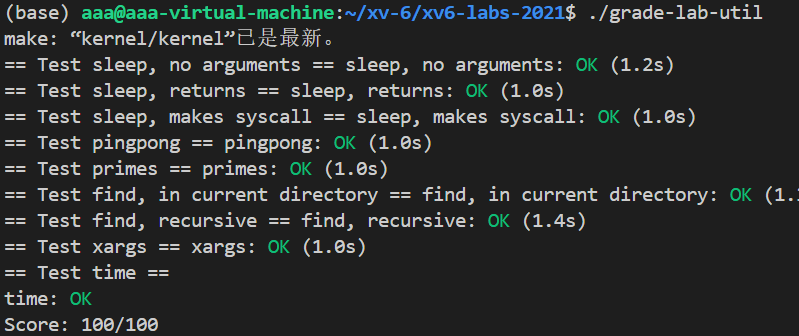
\includegraphics[width=\linewidth]{pics/util评测结果.png}
    \caption{评测结果}
    \label{fig:util}
\end{figure}

\subsection{实验小结}
本实验中我初步了解了xv6这个操作系统的基本结构。了解了其利用qemu模拟器运行、编程的基本方法。本实验中需要实现的多为基本的系统功能,让我对Unix操作系统有了更深入的了解。

此外primes是我认为这里面最难的程序。首先,理解这个程序的实现原理就花费了我不少时间。在之后实现这个程序的过程之中,我在处理管道、父子进程的关系的时候遇到了一些困难。不过最后我还是成功实现了程序,这对我理解管道、进程并行有很大的帮助。

\section{Lab: System calls}

\subsection{实验目的}

本实验旨在进一步熟悉系统调用,重点掌握如何添加系统调用,理解系统调用的工作原理,内核态和用户态的联系。

本实验实现了两个系统调用:
\begin{itemize}
    \item System call tracing:实现对系统调用的跟踪;
    \item Sysinfo:收集有关正在运行的系统的信息。
\end{itemize}

\subsection{实验步骤}

\subsubsection{实现trace}

\begin{enumerate}
    \item 首先,根据提示,在Makefile的UPROGS中添加\$U/\_trace\textbackslash。
    \item 在user.h文件的system calls部分添加trace函数。
          \newpage
          \begin{lstlisting}[language=c, title=对user.h的改动]
    // system calls
    int fork(void);
    ...
    // 添加 trace函数
    int trace(int);
    \end{lstlisting}
    \item 在usys.pl末尾添加entry("trace");以便在汇编语言中添加这个函数。
    \item 进入kernel文件夹,在syscall.h中添加SYS\_trace系统调用号的定义,值往下类推,即为22。
          \begin{lstlisting}[language=c, title=对syscall.h的更改]
    // System call numbers
    #define SYS_fork 1
    ...
    // 为trace添加系统调用号
    #define SYS_trace 22
          \end{lstlisting}
    \item 更改进程结构体。在proc.h中的进程结构体最后添加一个掩码trace\_mask,用于记录哪些进程要被追踪。
          \begin{lstlisting}[language=c, title=对进程结构体的更改]
    struct proc
    {
        struct spinlock lock;
        ...
        // 添加掩码
        int trace_mask;
    };
    \end{lstlisting}
    \item 在sysproc.c文件中,添加系统调用函数sys\_trace,在调用时设置掩码。
          \begin{lstlisting}[language=c, title=实现sys\_trace系统调用]
    uint64 sys_trace(void)
    {
        // 获取参数
        int mask;
        if (argint(0, &mask) < 0)
            return -1;
        // 获取当前进程
        struct proc *p = myproc();
        // 写入掩码
        p->trace_mask = mask;
        return 0;
    }
    \end{lstlisting}
    \item 在syscall.c中修改syscall函数,使其根据掩码判断是否输出当前调用信息。
          \begin{lstlisting}[language=c, title=对syscall函数的修改]
    void syscall(void)
    {
        int num;
        struct proc *p = myproc();

        num = p->trapframe->a7;
        if (num > 0 && num < NELEM(syscalls) && syscalls[num])
        {
            p->trapframe->a0 = syscalls[num]();

            // 获得掩码
            int trace_mask = p->trace_mask;

            // 如果掩码对应,输出当前系统调用信息
            if ((trace_mask >> num) & 1)
            {
                printf("%d: syscall %s -> %d\n", 
                        p->pid, 
                        syscall_names[num - 1], 
                        p->trapframe->a0);
            }
        }
        else
        {
            ...
        }
    }
    \end{lstlisting}
    \item 修改proc.c中的freeproc函数和fork函数,确保掩码在进程释放时重置掩码、在子进程创建时传递掩码。
          \newpage
          \begin{lstlisting}[language=c, title=对proc.c的修改]
    static void freeproc(struct proc *p)
    {
        if (p->trapframe)
        kfree((void *)p->trapframe);
        ...

        // 添加了这一行
        p->trace_mask = 0;
    }

    int fork(void)
    {
        ...

        // 把子进程的掩码也设置为与父进程相同
        np->trace_mask = p->trace_mask;

        ...
    }
    \end{lstlisting}
\end{enumerate}

\subsubsection{实现sysinfo}
\begin{enumerate}
    \item 首先,先仿照trace中的方法,在Makefile、syscall.h、syscall.c、user.h、user.pl中注册名为sysinfo的系统调用。
    \item 在kalloc.c中仿照kalloc函数读取空闲内存链表的方式,实现一个计算空闲内存空间大小的函数acquire\_freeman。
          \begin{lstlisting}[language=c, title=acquire\_freemem的实现]
    uint64 acquire_freemem()
    {
        struct run *r;
        uint64 cnt = 0;

        // 锁
        acquire(&kmem.lock);
        r = kmem.freelist;
        // 遍历链表
        while (r)
        {
            r = r->next;
            cnt++;
        }
        // 释放锁
        release(&kmem.lock);
        // 返回空间大小(页数乘页尺寸)
        return cnt * PGSIZE;
    }
    \end{lstlisting}
    \item 在proc.c中,实现一个计算非使用状态进程个数的函数acquire\_nproc,利用记录进程的数组struct proc proc[NPROC]。
          \begin{lstlisting}[language=c, title=acquire\_nproc的实现]
    uint64 acquire_nproc()
    {
        struct proc *p;
        int cnt = 0;
    
        for (p = proc; p < &proc[NPROC]; ++p)
        {
            acquire(&p->lock);
            if (p->state != UNUSED)
                cnt++;
            release(&p->lock);
        }
    
        return cnt;
    }    
    \end{lstlisting}
    \item 最后,在sysproc.c中完成sys\_sysinfo函数的实现。利用argaddr读取参数的地址,利用copyout对地址进行写入。
          \begin{lstlisting}[language=c, title=sys\_sysinfo的实现]
    uint64 sys_sysinfo(void)
    {
        struct sysinfo info;
        uint64 addr;
        struct proc *p = myproc();

        // 计算空闲进程数
        info.nproc = acquire_nproc();
        // 计算空闲内存数
        info.freemem = acquire_freemem();

        // 获取参数
        if (argaddr(0, &addr) < 0)
            return -1;
        // 写入结构体
        if (copyout(p->pagetable, addr, (char *)&info, sizeof(info)) < 0)
            return -1;
        return 0;
    }
    \end{lstlisting}
\end{enumerate}

\subsection{评测结果}
利用grade-lab-syscall脚本评测,得到评测结果如图\ref{fig:syscall}所示。
\begin{figure}[h]
    \centering
    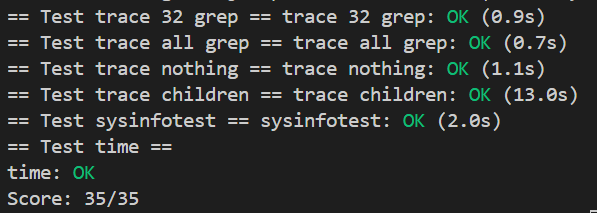
\includegraphics[width=\linewidth]{pics/syscall评测结果.png}
    \caption{评测结果}
    \label{fig:syscall}
\end{figure}

\subsection{实验小结}

在本实验中,我实现了两个系统调用。通过实验,我了解到了在内核中实现系统调用的一整套流程。

在实验中,为了实现我自己的系统调用,我阅读了许多kernel的代码,对内核有了更好的了解。通过仿照内核代码中一些函数的实现以及提示,我才得以完成我自己的系统调用。我在阅读内核代码的时候也遇到了一些困难,花费了不少时间来理解代码的含义。

这次实验大大加深了我对系统调用的了解,为之后的实验打下基础。


\section{Lab: Page tables}
\subsection{实验目的}

本实验中将涉及到操作系统中重要的\textbf{页表}概念。操作系统中的页表是一种数据结构,用于实现虚拟内存和物理内存之间的地址映射。每个进程都有自己的页表,将虚拟地址映射到物理地址,从而使得操作系统能够有效地管理内存,提供内存保护和共享内存功能。页表的概念对于操作系统课程至关重要,因为它涉及到内存管理、进程隔离和系统性能等核心问题。理解页表如何工作,有助于深入掌握操作系统的内存管理机制,了解虚拟内存的实现细节,并且能够解决与内存管理相关的各种问题。

本实验中将探索页表的具体操作并对其进行修改,以加快某些系统调用并检测哪些页面被访问。具体将实现以下内容:
\begin{itemize}
    \item 利用页表加速系统调用;
    \item 打印页表;
    \item 检测被访问的页表。
\end{itemize}

\subsection{实验步骤}

\subsubsection{实现系统调用加速}
\begin{enumerate}
    \item 首先,在proc.c文件中修改proc\_pagetable函数,仿照前面的代码添加用户页表的映射,注意内存权限应为PTE\_U。
          \begin{lstlisting}[language=c, title=对proc\_pagetable函数的修改]
    pagetable_t proc_pagetable(struct proc *p)
    {
        pagetable_t pagetable;

        ...

        // 添加的部分
        if (mappages(pagetable, USYSCALL, PGSIZE,
                    (uint64)(p->usyscall), PTE_R | PTE_U) < 0)
        {
            uvmunmap(pagetable, USYSCALL, 1, 0);
            uvmunmap(pagetable, TRAMPOLINE, 1, 0);
            uvmfree(pagetable, 0);
            return 0;
        }

        return pagetable;
    }
    \end{lstlisting}
    \item 在proc.c文件中修改allocproc函数,仿照前面的代码,给进程分配用户页表。
          \begin{lstlisting}[language=c, title=对allocproc函数的修改]
    static struct proc * allocproc(void)
    {
        ...
    
        // 添加的部分
        if ((p->usyscall = (struct usyscall *)kalloc()) == 0)
        {
            freeproc(p);
            release(&p->lock);
            return 0;
        }
        p->usyscall->pid = p->pid;
    
        ...

        return p;
    }
    \end{lstlisting}
    \item 在proc.c文件中修改freeproc函数,仿照前面的代码,释放用户页表。
          \begin{lstlisting}[language=c, title=对freeproc函数的修改]
    freeproc(struct proc *p)
    {
        ...
        // 添加的部分
        if (p->usyscall)
        kfree((void *)p->usyscall);
        p->usyscall = 0;
        ...
    }
    \end{lstlisting}
    \item 如此设置,系统就能利用用户页表实现更快地进程号查询,从而加速系统调用。
\end{enumerate}

\subsubsection{实现页表打印}
\begin{enumerate}
    \item 首先,阅读vm.c文件中freewalk函数的代码,了解如何对页表项进行递归遍历和访问。
          \begin{lstlisting}[language=c, title=freewalk函数的原型]
    // Recursively free page-table pages.
    // All leaf mappings must already have been removed.
    void freewalk(pagetable_t pagetable)
    {
        // there are 2^9 = 512 PTEs in a page table.
        for (int i = 0; i < 512; i++)
        {
            pte_t pte = pagetable[i];
            if ((pte & PTE_V) && (pte & (PTE_R | PTE_W | PTE_X)) == 0)
            {
                // this PTE points to a lower-level page table.
                uint64 child = PTE2PA(pte);
                freewalk((pagetable_t)child);
                pagetable[i] = 0;
            }
            else if (pte & PTE_V)
            {
                panic("freewalk: leaf");
            }
        }
        kfree((void *)pagetable);
    }
    \end{lstlisting}
    \item 仿照freewalk函数,实现递归打印页表的vmprint函数
          \begin{lstlisting}[language=c, title=vmprint函数的实现]
    void vmprint(pagetable_t pagetable, uint64 depth)
    {
        // 如果递归深度大于2,则直接返回,RISC-V只有三级页表
        if (depth > 2)
        return;
    
        // 如果是最顶层页表,打印页表的地址
        if (depth == 0)
        {
            printf("page table %p\n", pagetable);
        }
    
        // 定义一个静态的前缀数组,用于打印格式化输出
        static char *prefix[] = {"..", ".. ..", ".. .. .."};
    
        // 页表中有2^9 = 512个页表项
        for (int i = 0; i < 512; i++)
        {
            pte_t pte = pagetable[i];  // 获取当前页表项
            if (pte & PTE_V)  // 如果页表项有效
            {
                // 打印当前页表项的信息,包括前缀、索引、页表项和物理地址
                printf("%s%d: pte %p pa %p\n", prefix[depth], i, pte, PTE2PA(pte));
                uint64 child = PTE2PA(pte);  // 获取下一级页表的物理地址
                vmprint((pagetable_t)child, depth + 1);  // 递归打印下一级页表
            }
        }
    }
    \end{lstlisting}
    \item 在def.h中声明vmprint函数以便调用。
    \item 在exec.c文件中,对exec函数进行修改,调用vmprint函数,使其在进程号为1是打印页表。
          \begin{lstlisting}[language=c, title=对exec函数的修改]
    int exec(char *path, char **argv)
    {
        ...
        
        // 添加的语句
        if (p->pid == 1)
            vmprint(p->pagetable, 0);

        ...
    }    
    \end{lstlisting}
\end{enumerate}
\subsubsection{实现被访问页面侦测}
\begin{enumerate}
    \item 首先,在riscv.h文件中添加一个PTE\_A常量,查阅RISC-V手册可知其值应为0b00100000,即$2^6$。
          \begin{lstlisting}[language=c, title=PTE\_A的定义]
    #define PTE_A (1L << 6)    
    \end{lstlisting}
    \item 在vm.c文件中实现vm\_pgaccess函数,利用PTE\_A标志判断给定虚拟地址的页表项是否被访问,若被访问返回1并清除PTE\_A标志。在def.h中添加函数的声明。
          \begin{lstlisting}[language=c, title=vm\_pgaccess函数的实现]
    int vm_pgaccess(pagetable_t pagetable, uint64 va)
    {
        pte_t *pte;  // 页表项指针
    
        // 如果虚拟地址超出最大允许值,返回0
        if (va >= MAXVA)
            return 0;
    
        // 获取虚拟地址对应的页表项指针
        pte = walk(pagetable, va, 0);
        // 如果页表项不存在,返回0
        if (pte == 0)
            return 0;
    
        // 如果页表项的访问标志位被设置
        if ((*pte & PTE_A) != 0)
        {
            // 清除访问标志位
            *pte = *pte & (~PTE_A);
            // 返回1表示访问标志位被清除
            return 1;
        }
    
        // 如果访问标志位未设置,返回0
        return 0;
    }
    \end{lstlisting}
    \item 在sysproc.c中补全sys\_pgaccess系统调用,使之能够把页面访问的情况记录在掩码之中。
          \begin{lstlisting}[language=c, title=sys\_pgaccess函数的实现]
    int sys_pgaccess(void)
    {
        uint64 addr;  // 内存起始地址
        int len;      // 内存区域的页数
        int bitmask;  // 存储结果的用户地址
    
        // 获取系统调用的第一个参数(内存起始地址),并检查是否成功
        if (argaddr(0, &addr) < 0)
            return -1;
    
        // 获取系统调用的第二个参数(内存区域的页数),并检查是否成功
        if (argint(1, &len) < 0)
            return -1;
    
        // 获取系统调用的第三个参数(存储结果的用户地址),并检查是否成功
        if (argint(2, &bitmask) < 0)
            return -1;
    
        // 检查页数是否在合理范围内(0到32页)
        if (len > 32 || len < 0)
            return -1;
    
        int res = 0;  // 用于存储访问标志结果
        int i;
        struct proc *p = myproc();  // 获取当前进程结构体
    
        // 遍历每一页,检查访问标志并存储结果
        for (i = 0; i < len; i++)
        {
            int va = addr + i * PGSIZE;  // 计算每一页的虚拟地址
            int abit = vm_pgaccess(p->pagetable, va);  // 检查页表项的访问标志
        
            res = res | abit << i;  // 将访问标志结果合并到res中
        }
    
        // 将结果拷贝到用户空间,如果失败则返回-1
        if (copyout(p->pagetable, bitmask, (char *)&res, sizeof(res)) < 0)
            return -1;
    
        // 成功返回0
        return 0;
    }      
    \end{lstlisting}
\end{enumerate}

\subsection{评测结果}
利用 grade-lab-pgtbl 脚本评测,得到评测结果如图\ref{fig:pgtbl}所示。
\begin{figure}[h]
    \centering
    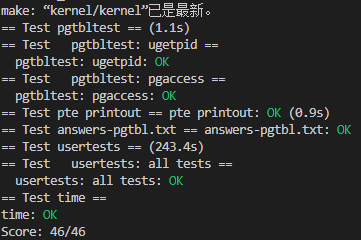
\includegraphics[width=\linewidth]{pics/pagetable评测结果.png}
    \caption{评测结果}
    \label{fig:pgtbl}
\end{figure}

\subsection{实验小结}
在本次实验中,我深入探索了操作系统中的页表概念,并通过一系列具体的实现来加深对该概念的理解。页表是操作系统中管理虚拟内存的重要数据结构,它通过将虚拟地址映射到物理地址,实现内存保护和内存共享功能。我通过本实验的操作,掌握了页表的操作方法和实现细节。

我在本实验上花费了不少时间,复习了操作系统课上讲过的页表概念,并研究内核代码。实验总体来说是有些难度。

在实验过程中,我不仅巩固了操作系统中页表的基本概念,还通过实际编程和调试,掌握了页表的具体实现方法和应用场景。通过这些实践操作,我更深入地理解了操作系统的内存管理机制,并积累了宝贵的编程经验和调试技巧。这些知识和技能对于我后续解决实际问题将大有裨益。


\section{Lab: Traps}

\subsection{实验目的}
这个实验将会探索系统调用是如何使用陷阱(trap)实现的。陷阱是一种特殊的处理机制,用于在计算机系统中捕获特定的事件或异常,并转移控制权给内核,从而确保系统能够安全地执行特权操作。理解陷阱机制对于掌握操作系统的核心功能和提升系统的安全性至关重要。实验内容具体包括:
\begin{itemize}
    \item 了解 RISC-V 程序集,阅读 call.asm 中的函数 g、f 和 main 的代码,了解基础的汇编知识,并回答问题。
    \item 实现一个回溯(backtrace)功能,用于在操作系统内核发生错误时,输出调用堆栈上的函数调用列表。这有助于调试和定位错误发生的位置。
    \item 添加系统调用 sigalarm,周期性地为进程设置定时提醒。
\end{itemize}

\subsection{实验步骤}
\subsubsection{了解 RISC-V 汇编}
首先,利用make fs.img命令对user文件夹下的call.c文件进行编译,并生成call.asm汇编文件。阅读 call.asm 中的 g ,f ,和 main 函数,并对给出的问题做出回答。
\begin{lstlisting}[language={[x86masm]Assembler}, title=call.asm]
    0000000000000000 <g>:
    #include "kernel/param.h"
    #include "kernel/types.h"
    #include "kernel/stat.h"
    #include "user/user.h"

    int g(int x) {
        0:	1141                	addi	sp,sp,-16
        2:	e422                	sd	s0,8(sp)
        4:	0800                	addi	s0,sp,16
        return x+3;
    }
    6:	250d                	addiw	a0,a0,3
    8:	6422                	ld	s0,8(sp)
    a:	0141                	addi	sp,sp,16
    c:	8082                	ret

    000000000000000e <f>:

    int f(int x) {
        e:	1141                	addi	sp,sp,-16
        10:	e422                	sd	s0,8(sp)
        12:	0800                	addi	s0,sp,16
        return g(x);
    }
    14:	250d                	addiw	a0,a0,3
    16:	6422                	ld	s0,8(sp)
    18:	0141                	addi	sp,sp,16
    1a:	8082                	ret

    000000000000001c <main>:

    void main(void) {
        1c:	1141                	addi	sp,sp,-16
        1e:	e406                	sd	ra,8(sp)
        20:	e022                	sd	s0,0(sp)
        22:	0800                	addi	s0,sp,16
        printf("%d %d\n", f(8)+1, 13);
        24:	4635                	li	a2,13
        26:	45b1                	li	a1,12
        28:	00000517          	auipc	a0,0x0
        2c:	7a050513          	addi	a0,a0,1952 # 7c8 <malloc+0xe8>
        30:	00000097          	auipc	ra,0x0
        34:	5f8080e7          	jalr	1528(ra) # 628 <printf>
        exit(0);
        38:	4501                	li	a0,0
        3a:	00000097          	auipc	ra,0x0
        3e:	274080e7          	jalr	628(ra) # 2ae <exit>
\end{lstlisting}

\subsubsection*{Q1: Which registers contain arguments to functions? For example, which register holds 13 in main's call to printf?}
答:RISC-V 中一共有 a0~a7 一共 8 个寄存器。在 main 函数调用 printf 函数的过程中,参数 13 被存储在了寄存器 a2 中。
\subsubsection*{Q2: Where is the call to function f in the assembly code for main? Where is the call to g?}

答:对于函数 f 调用是直接计算出了结果 12, 对于函数 g 的调用则是内联在了函数 f 中。

\subsubsection*{Q3: At what address is the function printf located?}

答:查阅代码可知printf函数的地址是0x628。
\begin{lstlisting}[language={[x86masm]Assembler}, title=printf函数]
    0000000000000628 <printf>:

    void
    printf(const char *fmt, ...)
    {
        628:	711d                	addi	sp,sp,-96
        62a:	ec06                	sd	ra,24(sp)
        62c:	e822                	sd	s0,16(sp)
        62e:	1000                	addi	s0,sp,32
        630:	e40c                	sd	a1,8(s0)
        632:	e810                	sd	a2,16(s0)
        634:	ec14                	sd	a3,24(s0)
        636:	f018                	sd	a4,32(s0)
        638:	f41c                	sd	a5,40(s0)
        63a:	03043823          	sd	a6,48(s0)
        63e:	03143c23          	sd	a7,56(s0)
        va_list ap;

        va_start(ap, fmt);
        642:	00840613          	addi	a2,s0,8
        646:	fec43423          	sd	a2,-24(s0)
        vprintf(1, fmt, ap);
        64a:	85aa                	mv	a1,a0
        64c:	4505                	li	a0,1
        64e:	00000097          	auipc	ra,0x0
        652:	dce080e7          	jalr	-562(ra) # 41c <vprintf>
    }
    656:	60e2                	ld	ra,24(sp)
    658:	6442                	ld	s0,16(sp)
    65a:	6125                	addi	sp,sp,96
    65c:	8082                	ret
\end{lstlisting}

\subsubsection*{Q4: What value is in the register ra just after the jalr to printf in main?}

答:把运行到jalr处的PC+4存入ra,也就是0x38。

\subsubsection*{Q5: Run the following code. What is the output? The output depends on that fact that the RISC-V is little-endian. If the RISC-V were instead big-endian what would you set i to in order to yield the same output? Would you need to change 57616 to a different value?}
\begin{lstlisting}[language=c, title=Code for Question]
    unsigned int i = 0x00646c72;
    printf("H%x Wo%s", 57616, &i);
\end{lstlisting}

答:程序的输出是He110 World。如果是大端序(big-endian),那么i应该设置为0x726c6400 才能保证与小端序输出的内容相同,即“rld”。57616是不需要改的,因为其十六进制无论大小端都为0xe110。

\subsubsection*{Q6: In the following code, what is going to be printed after 'y='? Why does this happen?}
\begin{lstlisting}[language=c, title=Code for Question]
    printf("x=%d y=%d", 3);
\end{lstlisting}

答:它所输出的是寄存器 a2 的值,这是因为 printf 会从 a2 寄存器读取参数作为
y 的值。其具体值受先前调用的影响。

\subsubsection{实现 Backtrace}
\begin{enumerate}
    \item 首先,在defs.h中添加backtrace函数的声明。
          \begin{lstlisting}[language=c, title=backtrace函数的声明]
    void backtrace(void);
    \end{lstlisting}
    \item 根据题目要求,在riscv.c文件中添加一个r\_fp函数,用于获取栈帧。
          \begin{lstlisting}[language=c, title=r\_fp函数的实现]
    static inline uint64 r_fp()
    {
        uint64 x;
        asm volatile("mv %0, s0" : "=r"(x));
        return x;
    }
    \end{lstlisting}
    \item 在printf.c文件中添加backtrace函数的实现。
          \begin{lstlisting}[language=c, title=backtrace函数的实现]
    void backtrace(void)
    {
        printf("backtrace:\n");

        // 获取当前栈帧指针
        uint64 fp = r_fp();

        // 计算当前栈帧指针所在页的起始地址
        uint64 base = PGROUNDUP(fp);

        // 当栈帧指针小于页的起始地址时,继续回溯
        while (fp < base)
        {
            // 打印前一个栈帧的返回地址
            printf("%p\n", *((uint64 *)(fp - 8)));

            // 更新栈帧指针为前一个栈帧的指针
            fp = *((uint64 *)(fp - 16));
        }
    }
    \end{lstlisting}
\end{enumerate}

\subsubsection{实现alarm}
\begin{enumerate}
    \item 首先,修改user.pl、user.h、syscall.h、syscall.c,添加两个系统调用sigalarm和sigreturn,方法与前文相同。sigreturn不接受任何参数,而sigalarm为int sigalarm(int ticks, void (*handler)())。
    \item 修改proc.h中的进程结构体,添加一些新成员,用于记录程序的中断信息。
          \begin{lstlisting}[language=c, title=对进程结构体的修改]
    struct proc
    {
        ...

        int ticks; // 记录进程运行的tick
        int ticks_cnt; // tick计数
        uint64 handler; // 处理程序的入口地址
        struct trapframe tick_trapframe; // 记录进程运行上下文
        int handler_executing; // 记录当前处理程序是否允许的状态量
    };
    \end{lstlisting}
    \item 修改proc.c中的allocproc函数,添加对结构体新成员的初始化。
          \begin{lstlisting}[language=c,title=对allocproc函数的修改]
    static struct proc *
    allocproc(void)
    {
        ...

        p->ticks = 0;
        p->handler_executing = 0;

        return p;
    }
    \end{lstlisting}
    \item 在sysproc.c中添加sigalarm和sigreturn函数的实现。实现中断程序的跳转和恢复。
          \begin{lstlisting}[language=c,title=sys\_sigalarm的实现]
    uint64 sys_sigalarm(void)
    {
        int ticks;           // 定义变量ticks,用于存储定时器的滴答数
        uint64 handler;      // 定义变量handler,用于存储信号处理函数的地址

        // 获取第一个参数的值并赋给ticks
        argint(0, &ticks);   
        // 获取第二个参数的值并赋给handler
        argaddr(1, &handler);

        // 获取当前进程的指针
        struct proc *p = myproc();
        // 设置当前进程的定时器滴答数
        p->ticks = ticks;
        // 设置当前进程的信号处理函数
        p->handler = handler;
        // 初始化滴答计数器为0
        p->ticks_cnt = 0;

        // 返回0,表示成功
        return 0;
    }
    \end{lstlisting}
          \newpage
          \begin{lstlisting}[language=c,title=sys\_sigreturn的实现]
    // 定义sys_sigreturn函数,返回类型为uint64
    uint64 sys_sigreturn(void)
    {
        // 获取当前进程的指针
        struct proc *p = myproc();
    
        // 将当前进程的trapframe恢复为tick_trapframe
        *(p->trapframe) = p->tick_trapframe;
    
        // 设置handler_executing为0,表示处理函数执行完毕
        p->handler_executing = 0;
        
        // 返回0,表示成功
        return 0;
    }
        \end{lstlisting}
    \item 修改trap.c文件中的usertrap函数,定义操作系统处理中断的行为。
          \begin{lstlisting}[language=c,title=对usertrap函数的修改]
    void usertrap(void)
    {
        ...

        // 如果这是一个时钟中断,则可能需要让出 CPU
        if (which_dev == 2)
        {
            // 检查进程是否设置了定时器
            if (p->ticks > 0)
            {
                p->ticks_cnt++;  // 增加定时器计数

                // 如果信号处理程序未在执行中且计数器超过了设定的滴答数
                if (p->handler_executing == 0 && p->ticks_cnt > p->ticks)
                {
                    p->ticks_cnt = 0;  // 重置计数器
                    p->tick_trapframe = *(p->trapframe);  // 保存当前的 trapframe
                    p->trapframe->epc = p->handler;  // 设置程序计数器为信号处理程序的地址
                    p->handler_executing = 1;  // 标记信号处理程序正在执行
                }
            }

            // 放弃 CPU,使其他进程能够运行
            yield();
        }

        // 恢复到用户模式继续执行
        usertrapret();
    }
    \end{lstlisting}
\end{enumerate}
\subsection{评测结果}
利用 grade-lab-traps 脚本评测,得到评测结果如图\ref{fig:traps}所示。
{fig:syscall}所示。
\begin{figure}[h]
    \centering
    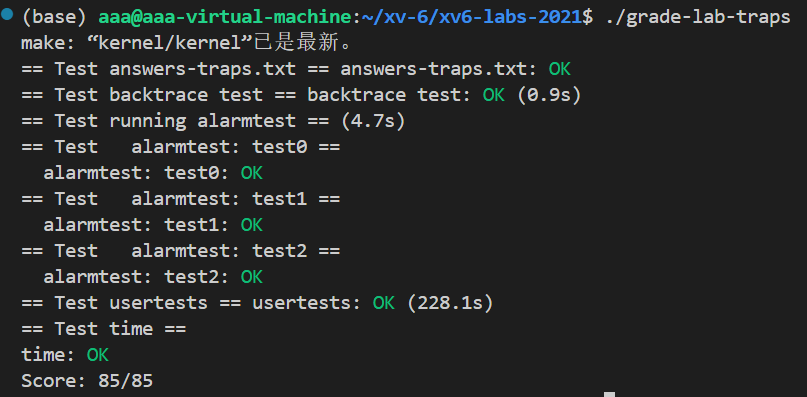
\includegraphics[width=\linewidth]{pics/traps评测结果.png}
    \caption{评测结果}
    \label{fig:traps}
\end{figure}


\subsection{实验小结}
本次实验通过实现系统调用和陷阱机制,深入理解了操作系统的核心功能。

这些操作增强了我对计算机体系结构、异常处理机制和系统调用流程的理解。通过实际编写和测试系统调用,我更好地理解了用户态和内核态之间的交互机制,以及系统调用是如何在硬件和操作系统之间传递控制权的。实现陷阱机制和backtrace功能,使我熟悉了如何捕获和处理异常,以及如何在错误发生时进行有效的调试和错误定位。添加定时提醒功能(sigalarm)使我了解了如何在操作系统中实现高级特性,从而提高系统的可用性和可靠性。通过设置定时器,可以更好地理解系统中断。

总的来说,本次实验不仅增强了我对操作系统原理的理解,还提升了我在实际系统开发中的调试和错误处理能力。


\section{Lab: Copy-on-Write Fork for xv6}
\subsection{实验目的}

本实验旨在促进了解写时复制(Copy-On-Write,COW)机制,同时增进对fork函数分配内存机制的理解。在 xv6 操作系统内核中实现COW机制。通过实现 COW 机制,可以在fork 系统调用时避免直接复制父进程的所有内存页,从而提高内存使用效率。当子进程尝试写入共享页面时,再复制相应的页面。

\subsection{实验步骤}

\begin{enumerate}
    \item 首先,修改riscv.h文件,添加一个页表标志位PTE\_COW,用于记录页表是否处于COW状态。
          \begin{lstlisting}[language=c,title=对riscv.h文件的修改]
    #define PTE_V (1L << 0) // valid
    #define PTE_R (1L << 1)
    #define PTE_W (1L << 2)
    #define PTE_X (1L << 3)
    #define PTE_U (1L << 4) // 1 -> user can access
    #define PTE_COW (1L << 8) // 1 -> cow page
    \end{lstlisting}
    \item 在kalloc.c文件中添加一个数组int reference[PHYSTOP / PGSIZE]记录页表引用数,并设置一个锁确保对数组的安全操作。
          \begin{lstlisting}[language=c,title=添加记录引用数的数组和锁]
    int reference[PHYSTOP / PGSIZE];
    struct spinlock refcountlock;
    \end{lstlisting}
    \item 修改kalloc函数和kfree函数,实现对reference数组的初始化和页面释放。
          \begin{lstlisting}[language=c,title=对kalloc函数的修改]
    void *kalloc(void)
    {
        struct run *r;

        acquire(&kmem.lock);
        r = kmem.freelist;
        
        // 如果有空闲页面,分配给请求者
        if (r)
        {
            kmem.freelist = r->next;
            // 添加部分
            acquire(&refcountlock);
            reference[((uint64)r) / PGSIZE] = 1;
            release(&refcountlock);
        }
        release(&kmem.lock);

        if (r)
            memset((char *)r, 5, PGSIZE); // fill with junk
        return (void *)r;
    }
    \end{lstlisting}
          \begin{lstlisting}[language=c,title=对kfree函数的修改]
    void kfree(void *pa)
    {
        struct run *r;
        
        if (((uint64)pa % PGSIZE) != 0 
        || (char *)pa < end 
        || (uint64)pa >= PHYSTOP)
            panic("kfree");

        // 添加部分,减少引用计数
        acquire(&refcountlock);
        reference[((uint64)pa) / PGSIZE]--;
        release(&refcountlock);
        if (reference[((uint64)pa) / PGSIZE] > 0)
            return;

        // Fill with junk to catch dangling refs.
        memset(pa, 1, PGSIZE);

        r = (struct run *)pa;

        acquire(&kmem.lock);
        r->next = kmem.freelist;
        kmem.freelist = r;
        release(&kmem.lock);
    } 
    \end{lstlisting}
    \item 修改trap.c文件,添加一个cowhandler函数并修改usertrap函数,当发生缺页异常,为进程复制一个新物理页面。
          \begin{lstlisting}[language=c,title=cowhandler函数的实现]
    int cowhandler(pagetable_t pagetable, uint64 va)
    {
        char *mem;
    
        // 检查虚拟地址是否超过最大有效地址
        if (va >= MAXVA)
            return -1;
        // 获取页表条目(PTE)
        pte_t *pte = walk(pagetable, va, 0);
        if (pte == 0)
            return -1;   
        // 检查PTE是否有效、用户模式、COW标志
        if ((*pte & PTE_V) == 0 || (*pte & PTE_U) == 0 || (*pte & PTE_COW) == 0)
            return -1;
        // 分配一个新的物理页面
        if ((mem = kalloc()) == 0)
            return -1; 
        // 获取原物理地址
        uint64 pa = PTE2PA(*pte);
        // 将原物理页面内容复制到新页面
        memmove((char *)mem, (char *)pa, PGSIZE);
        // 释放原物理页面
        kfree((void *)pa);
        // 获取PTE的标志位
        uint flags = PTE_FLAGS(*pte);
        // 更新PTE指向新物理页面,并设置为可写
        *pte = (PA2PTE(mem) | flags | PTE_W);
        // 清除COW标志
        *pte &= ~PTE_COW;
    
        return 0;
    }            
    \end{lstlisting}
          \begin{lstlisting}[language=c,title=对usertrap函数的修改]
    void usertrap(void)
    {
        ...

        // 检查陷阱原因
        if (r_scause() == 8)
        {
            ...
        }
        else if (r_scause() == 15)
        {
            // 处理Copy-On-Write(COW)错误
            uint64 va = r_stval();
            if (va >= p->sz)
                p->killed = 1;
            int ret = cowhandler(p->pagetable, va);
            if (ret != 0)
                ->killed = 1;
        }
        else if ((which_dev = devintr()) != 0)
        {
            // 设备中断
            // ok
        }
        else
        {
            ...
        }

        ...
        
        usertrapret();
    }
    \end{lstlisting}
    \item 在vm.c文件中修改copyout函数,添加COW页面的处理逻辑。
          \begin{lstlisting}[language=c,title=对copyout函数的修改]
    int copyout(pagetable_t pagetable, uint64 dstva, char *src, uint64 len)
    {
        uint64 n, va0, pa0;

        while (len > 0)
        {
            ...

            // 如果是Copy-On-Write页面,处理COW逻辑
            if (checkcowpage(va0, pte, p))
            {
                char *mem;

                // 分配一个新的物理页面
                if ((mem = kalloc()) == 0)
                {
                    p->killed = 1;
                }
                else
                {
                    // 将原页面的数据复制到新页面
                    memmove(mem, (char *)pa0, PGSIZE);

                    // 获取页表条目的标志位
                    uint flags = PTE_FLAGS(*pte);

                    // 解除原页面映射
                    uvmunmap(pagetable, va0, 1, 1);

                    // 更新页表条目,指向新页面并设置为可写
                    *pte = (PA2PTE(mem) | flags | PTE_W);

                    // 清除COW标志
                    *pte &= ~PTE_COW;

                    // 更新物理地址
                    pa0 = (uint64)mem;
                }
            }

            ...
        }

        return 0;
    }
    \end{lstlisting}
\end{enumerate}

\subsection{评测结果}
利用grade-lab-cow脚本评测,得到结果如图\ref{fig:cow}。
\begin{figure}[h]
    \centering
    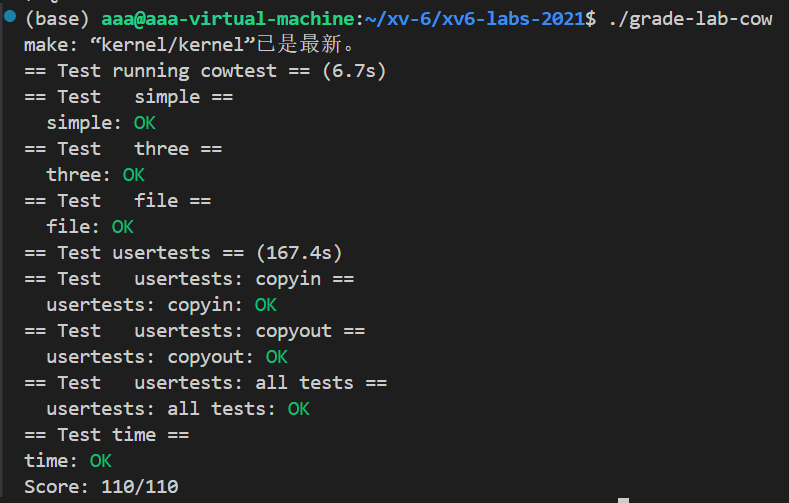
\includegraphics[width=\linewidth]{pics/cow评测结果.png}
    \caption{评测结果}
    \label{fig:cow}
\end{figure}

\subsection{实验小结}
本次实验通过在 xv6 操作系统内核中实现写时复制(Copy-On-Write,COW)机制,加深了我对内存管理和进程创建的理解。在传统的fork系统调用中,父进程的所有内存页都会被直接复制给子进程,而COW机制通过延迟实际的内存复制操作,提高了内存使用效率。

通过实验,我不仅掌握了COW机制的基本原理,还增强了对操作系统内存管理和进程管理的理解,提升了在操作系统内核中进行实际编程和调试的能力。这些技能对于理解和开发高效的操作系统具有重要意义。


\section{Lab: Multithreading}

\subsection{实验目的}
本实验旨在进一步了解多线程编程,在操作系统中实现线程执行和切换等操作。实验将在用户级线程包中实现线程之间的切换,使用多个线程来加速程序,并实现barrier。

\subsection{实验步骤}
\subsubsection{实现用户线程切换}
\begin{enumerate}
    \item 修改uthread.c文件:
          \begin{itemize}
              \item 添加一个context结构体保存线程上下文的寄存器。
                    \begin{lstlisting}[language=c,title=context结构体]
    struct context
    {
        uint64 ra;
        uint64 sp;

        uint64 s0;
        uint64 s1;
        uint64 s2;
        uint64 s3;
        uint64 s4;
        uint64 s5;
        uint64 s6;
        uint64 s7;
        uint64 s8;
        uint64 s9;
        uint64 s10;
        uint64 s11;
    };
    \end{lstlisting}
              \item 在thread结构体中添加一个保存上下文的context结构体成员。
                    \begin{lstlisting}[language=c,title=对thread结构体的修改]
    struct thread
    {
        char stack[STACK_SIZE]; 
        int state;              
        struct context context; /* 线程上下文 */
    };
        \end{lstlisting}

              \item 修改thread\_schedule函数实现线程切换。
                    \begin{lstlisting}[language=c,title=对thread\_schedule函数的修改]
    void thread_schedule(void)
    {
        struct thread *t, *next_thread;
    
        ...
    
        if (current_thread != next_thread)  // 如果需要切换线程
        {
            next_thread->state = RUNNING;  // 设置下一个线程为运行状态
            t = current_thread;  // 保存当前线程
            current_thread = next_thread;  // 切换到下一个线程
            // 切换线程上下文
            thread_switch((uint64)&t->context, (uint64)&next_thread->context);  
        }
        else
            next_thread = 0;  // 如果没有切换线程,则将next_thread置为0
    }            
              \end{lstlisting}
              \item 修改thread\_create函数初始化context结构体,设置栈顶指针和函数指针。
                    \begin{lstlisting}[language=c,title=对thread\_create函数的修改]
    void thread_create(void (*func)())
    {
        struct thread *t;

        for (t = all_thread; t < all_thread + MAX_THREAD; t++)  // 查找空闲的线程结构
        {
            if (t->state == FREE)  // 如果找到空闲线程
                break;  // 跳出循环
        }
        t->state = RUNNABLE;  // 设置线程状态为可运行

        //添加的部分
        t->context.sp = (uint64)&t->stack + STACK_SIZE;  // 初始化线程栈顶指针
        t->context.ra = (uint64)func;  // 设置返回地址为函数指针
    }
            \end{lstlisting}
          \end{itemize}

    \item 修改uthread\_switch.S文件,实现thread\_switch函数,保存当前线程的寄存器并恢复新线程的寄存器。
          \begin{lstlisting}[language={[x86masm]Assembler},title=实现thread\_switch汇编]
        thread_switch:
            sd ra, 0(a0)
            sd sp, 8(a0)
            sd s0, 16(a0)
            sd s1, 24(a0)
            sd s2, 32(a0)
            sd s3, 40(a0)
            sd s4, 48(a0)
            sd s5, 56(a0)
            sd s6, 64(a0)
            sd s7, 72(a0)
            sd s8, 80(a0)
            sd s9, 88(a0)
            sd s10, 96(a0)
            sd s11, 104(a0)
            ld ra, 0(a1)
            ld sp, 8(a1)
            ld s0, 16(a1)
            ld s1, 24(a1)
            ld s2, 32(a1)
            ld s3, 40(a1)
            ld s4, 48(a1)
            ld s5, 56(a1)
            ld s6, 64(a1)
            ld s7, 72(a1)
            ld s8, 80(a1)
            ld s9, 88(a1)
            ld s10, 96(a1)
            ld s11, 104(a1)
            ret    /* return to ra */
        \end{lstlisting}
\end{enumerate}

\subsubsection{使用 UNIX pthread 线程库实现一个线程安全的哈希表}
这部分实现不需要使用xv6操作系统部分的代码。首先观察ph.c文件,编译运行,发现程序在单线程运行时,哈希表没有出现丢失key的情况,而在双线程运行时就会发生丢失key的情况。经过观察,发现put函数中的插入操作不是线程安全的,通过为这部分代码加入互斥锁便可解决问题。

\begin{enumerate}
    \item 在全局变量中加入一个互斥锁。
          \begin{lstlisting}[language=c,title=声明互斥锁]
    struct entry *table[NBUCKET];
    int keys[NKEYS];
    int nthread = 1;
    // 添加的互斥锁
    pthread_mutex_t lock[NBUCKET];
    \end{lstlisting}
    \item 在main函数的开头初始化互斥锁。
          \begin{lstlisting}[language=c,title=初始化互斥锁]
    int main(int argc, char *argv[])
    {
        ...
    
        for (int i = 0; i < NBUCKET; i++)
        {
            pthread_mutex_init(&lock[i], NULL);
        }
    
        ...
    }
    \end{lstlisting}
    \item 在put函数中使用互斥锁,确保线程安全。
          \begin{lstlisting}[language=c,title=对put函数的修改]
    static void put(int key, int value)
    {
        int i = key % NBUCKET;

        // is the key already present?
        struct entry *e = 0;
        for (e = table[i]; e != 0; e = e->next)
        {
            if (e->key == key)
                break;
        }
        if (e)
        {
            // update the existing key.
            e->value = value;
        }
        else
        {
            // 添加互斥锁
            pthread_mutex_lock(&lock[i]);
            insert(key, value, &table[i], table[i]);
            pthread_mutex_unlock(&lock[i]);
        }
    }
    \end{lstlisting}
\end{enumerate}

\subsubsection{实现barrier}
barrier 函数的作用是在并发编程中同步多个线程,使得它们在某个点上等待,直到所有线程都到达该点,然后再继续执行。这确保了所有线程在某个阶段结束前不会提前进入下一个阶段。

\begin{lstlisting}[language=c,title=对barrier函数的实现]
    static void barrier() 
    {
        pthread_mutex_lock(&bstate.barrier_mutex);  // 加锁保护屏障状态

        bstate.nthread++;  // 已到达屏障的线程数加1

        if (bstate.nthread == nthread) 
        {  // 如果所有线程都到达屏障
            bstate.nthread = 0;  // 重置已到达线程数
            bstate.round++;  // 增加屏障轮次
            pthread_cond_broadcast(&bstate.barrier_cond);  // 唤醒所有等待线程
        } 
        else 
        {
            // 等待其他线程到达屏障
            pthread_cond_wait(&bstate.barrier_cond, &bstate.barrier_mutex);  
        }

        pthread_mutex_unlock(&bstate.barrier_mutex);  // 解锁
    }

\end{lstlisting}

\subsection{评测结果}
利用grade-lab-thread脚本评测,得到结果如图\ref{fig:thread}所示。
\begin{figure}[h]
    \centering
    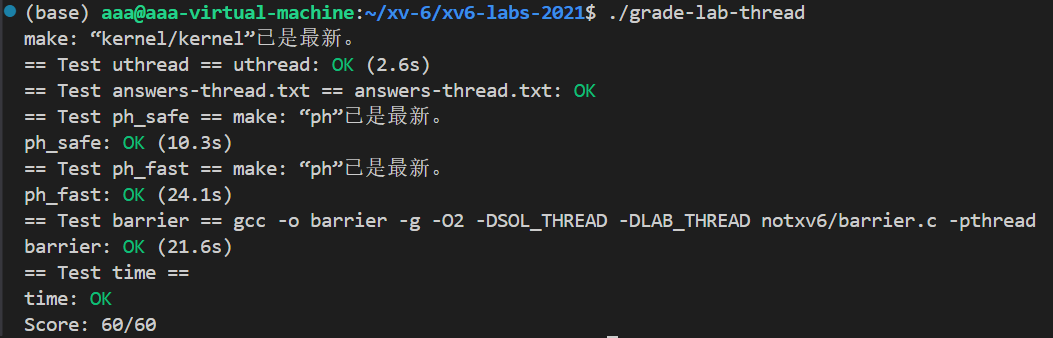
\includegraphics[width=\linewidth]{pics/thread评测结果.png}
    \caption{评测结果}
    \label{fig:thread}
\end{figure}

\subsection{实验小结}

\subsubsection*{为什么使用单线程运行哈希表就不会丢失key,而双线程就会丢失?}
有两个线程时,缺失键的问题是因为存在竞态条件。多个线程同时访问和修改共享数据(哈希表)时,会导致不可预测的结果。例如,线程1和线程2同时检查同一个桶,并发现键不存在,随后都尝试插入该键,这会导致其中一个插入操作被覆盖,从而导致缺失键。使用互斥锁(mutex)来保护对哈希表的访问可以解决这个问题。
\subsubsection*{总结}
本次实验深入探讨了多线程编程的实现与应用,涵盖了用户级线程切换、线程安全数据结构以及同步机制的实现。通过这些实现,我们不仅掌握了多线程编程的基本技术,还理解了线程同步和数据一致性的重要性。这些技能对于开发高效、可靠的并发程序具有重要意义。本实验为将来的复杂系统开发奠定了坚实基础。

\section{Lab: Networking}

\subsection{实验目的}

本实验将编写一个在xv6操作系统中用于网络接口卡(network interface card, NIC)的设备驱动程序。通过这个实验学习如何初始化并操作一个虚拟的网络设备,以及如何处理网络通信,从而深入理解操作系统中设备驱动程序的工作原理。

本实验将使用一个名为 E1000 的网络设备来处理网络通信。对于 xv6来说,E1000 看起来就像一个连接到真实以太网局域网(LAN)的真实硬件。

\subsection{实验步骤}

在e1000.c文件中完善e1000\_transmit和e1000\_recv函数以实现网卡驱动的功能。

\subsubsection*{e1000\_transmit函数}
e1000\_transmit 函数的作用是将一个数据缓冲区(mbuf)通过 e1000 网卡发送出去。它首先获取一个自旋锁以确保线程安全,然后读取当前的发送描述符索引(TDT)。接着检查对应的发送描述符是否已经被处理,如果未处理则返回错误。否则,将新数据缓冲区的地址和长度写入发送描述符,并设置相关的命令和状态位,通知网卡发送该数据包。最后,更新发送描述符索引(TDT),释放锁并返回成功标志。


\begin{lstlisting}[language=c,title=e1000\_transmit函数的实现]
    int e1000_transmit(struct mbuf *m)
    {
        // 获取e1000锁,确保对发送环形缓冲区的访问是安全的
        acquire(&e1000_lock);

        // 获取当前TDT(发送描述符尾部指针)的值,即网卡硬件当前处理到的发送描述符索引
        uint64 tdt = regs[E1000_TDT];
        // 计算发送环中的当前索引
        uint64 index = tdt % TX_RING_SIZE;
        // 获取当前索引处的发送描述符
        struct tx_desc send_desc = tx_ring[index];

        // 检查发送描述符是否已经被硬件处理(通过判断状态位是否包含DD标志)
        if (!(send_desc.status & E1000_TXD_STAT_DD))
        {
            // 如果发送描述符尚未处理,说明环形缓冲区满,释放锁并返回-1表示失败
            release(&e1000_lock);
            return -1;
        }

        // 如果之前存在缓冲区,则释放它
        if (tx_mbufs[index] != 0)
        {
            mbuffree(tx_mbufs[index]);
        }

        // 将新的缓冲区指针存储到对应位置
        tx_mbufs[index] = m;
        // 将缓冲区的地址写入描述符
        tx_ring[index].addr = (uint64)tx_mbufs[index]->head;
        // 将缓冲区的长度写入描述符
        tx_ring[index].length = (uint16)tx_mbufs[index]->len;
        // 设置描述符的命令位,指示这是一个要发送的完整数据包,并要求发送后更新状态
        tx_ring[index].cmd = E1000_TXD_CMD_RS | E1000_TXD_CMD_EOP;
        // 清除描述符的状态位,准备发送
        tx_ring[index].status = 0;

        // 更新TDT寄存器,使网卡处理下一个发送描述符
        tdt = (tdt + 1) % TX_RING_SIZE;
        regs[E1000_TDT] = tdt;
        // 确保所有内存操作在同步点前完成
        __sync_synchronize();

        // 释放e1000锁
        release(&e1000_lock);

        // 返回0表示发送操作已成功提交
        return 0;
    }

\end{lstlisting}

\subsubsection*{e1000\_recv函数}
e1000\_recv 函数的作用是处理网卡接收到的数据包。它首先读取当前的接收描述符索引(RDT),计算下一个接收描述符的位置。然后检查接收描述符的状态位,以确定是否有新的数据包到达。如果有数据包到达,函数会将数据从接收描述符复制到相应的缓冲区(mbuf),并调用上层的网络处理函数(net\_rx)处理数据包。接着,分配新的缓冲区并更新接收描述符,以便网卡继续接收新的数据。最后,更新接收描述符索引(RDT),以通知网卡新的描述符可用。

\begin{lstlisting}[language=c,title=e1000\_recv函数的实现]
    static void e1000_recv(void)
    {
        // 获取当前RDT(接收描述符尾部指针)的值,即网卡硬件当前处理到的接收描述符索引
        uint64 rdt = regs[E1000_RDT];
        // 计算接收环中下一个描述符的索引
        uint64 index = (rdt + 1) % RX_RING_SIZE;

        // 检查当前接收描述符的状态位是否包含DD标志,即是否有数据包到达
        if (!(rx_ring[index].status & E1000_RXD_STAT_DD))
        {
            // 如果没有数据包到达,直接返回
            return;
        }

        // 使用while循环处理所有可用的数据包
        while (rx_ring[index].status & E1000_RXD_STAT_DD)
        {
            // 获取当前索引处的mbuf指针
            struct mbuf *buf = rx_mbufs[index];
            // 将数据包长度写入mbuf并调整指针
            mbufput(buf, rx_ring[index].length);
            // 为接收环形缓冲区分配新的mbuf
            rx_mbufs[index] = mbufalloc(0);
            // 如果分配失败,则触发panic(此处不在代码中实现)
            // 更新接收描述符的地址字段,以便接收新数据包
            rx_ring[index].addr = (uint64)rx_mbufs[index]->head;
            // 清除描述符的状态位,准备接收下一个数据包
            rx_ring[index].status = 0;
            // 更新RDT寄存器,指示网卡可以使用这个描述符
            rdt = index;
            regs[E1000_RDT] = rdt;
            // 确保所有内存操作在同步点前完成
            __sync_synchronize();

            // 调用网络层处理函数,将数据包传递到更高层处理
            net_rx(buf);
            // 计算下一个描述符的索引
            index = (regs[E1000_RDT] + 1) % RX_RING_SIZE;
        }
    }
\end{lstlisting}

\subsection{评测结果}
利用grade-lab-cow脚本评测,得到结果如图\ref{fig:net}。
\begin{figure}[h]
    \centering
    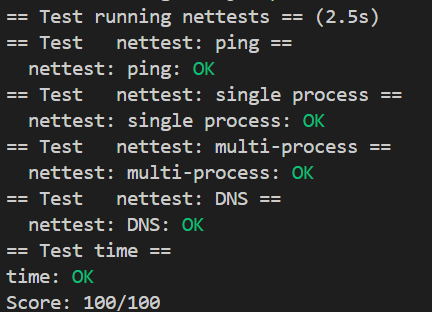
\includegraphics[width=\linewidth]{pics/net评测结果.png}
    \caption{评测结果}
    \label{fig:net}
\end{figure}

\subsection{实验小结}

通过本次实验,我成功实现了在xv6操作系统中对E1000网络设备的驱动程序编写。具体实现了数据包的发送(e1000\_transmit函数)和接收(e1000\_recv函数)功能。这一过程加深了我对设备驱动程序工作原理的理解,尤其是在网络通信中的应用。

整个实验过程中,我不仅掌握了如何编写和调试设备驱动程序,还通过实际操作理解了操作系统中网络通信的底层机制。这些经验和知识为我今后开发复杂的系统级软件奠定了坚实的基础。同时,通过评测脚本验证了我实现的正确性,确保了驱动程序的功能和性能达到了预期的目标。

\section{Lab: Locks}

\subsection{实验目的}
本实验将重新设计代码以提高并行性。多核机器上并行性差的一个常见症状是高锁争用。提高并行性通常涉及更改数据结构和锁定策略以减少争用。实验将为 xv6 内存分配器和块缓存执行此操作。

\subsection{实验步骤}

\subsubsection{优化Memory allocator}

修改系统对内存的管理方式。修改后,物理内存的分配和释放通过一系列链表进行管理,这些链表称为空闲链表(freelist),每个链表节点代表一块空闲的物理内存。

系统为每个 CPU 分配了一个单独的空闲链表,并为每个链表分配了一个自旋锁,以确保在多核环境下的同步操作。每当内存需要释放时,内存管理器会将内存块插入到相应 CPU 的空闲链表的头部。这个操作受 CPU 的自旋锁保护,以避免在并发情况下的数据竞争。内存分配时,首先会尝试从当前 CPU 的空闲链表中获取空闲页面,如果当前 CPU 的链表为空,则尝试从其他 CPU 的链表中窃取一个页面。

具体来说,就是对kalloc.c文件进行修改,以应用这种内存管理的方式。修改如下:
\begin{enumerate}
    \item 修改kmem结构体,把它改为数组的形式,以便将其拆分到每个CPU中。
          \begin{lstlisting}[language=c,title=对kmem结构体的修改]
    // kmem 是一个包含 NCPU 个元素的数组,每个元素对应一个 CPU 的物理内存管理结构。
    // 其中 lock 是自旋锁,用于保护空闲链表 freelist。
    struct
    {
        struct spinlock lock; // 自旋锁,用于多核环境下的同步。
        struct run *freelist; // 空闲链表,指向空闲内存块。
    } kmem[NCPU];           // 定义 NCPU 个这样的结构体数组。
    \end{lstlisting}
    \item 修改kinit函数,初始化空闲链表。
          \begin{lstlisting}[language=c,title=对kinit函数的修改]
    // 初始化内存分配器
    void kinit()
    {
        char lockname[16]; // 用于存储锁的名字。
        for (int i = 0; i < NCPU; i++)
        {
        // 为每个 CPU 初始化一个自旋锁,并给它们命名。
        snprintf(lockname, sizeof(lockname), "kmem_CPU%d", i);
        initlock(&kmem[i].lock, lockname);
        }
        // 将从内核结束位置(end)到物理内存顶(PHYSTOP)之间的内存标记为空闲。
        freerange(end, (void *)PHYSTOP);
    }    
    \end{lstlisting}
    \item 修改kfree,把释放后的内存加入空闲链表。
          \begin{lstlisting}[language=c,title=对kfree函数的修改]
    void kfree(void *pa)
    {
        struct run *r; // 临时指针,用于指向将要释放的内存块。
        int cpu_id;    // 存储当前 CPU 的 ID。
    
        // 如果 pa 不是页面对齐的,或地址超出合法范围,则触发 panic。
        if (((uint64)pa % PGSIZE) != 0 || (char *)pa < end || (uint64)pa >= PHYSTOP)
        panic("kfree");
    
        // 将内存填充为 1,以捕捉潜在的悬空引用(dangling references)。
        memset(pa, 1, PGSIZE);
    
        r = (struct run *)pa; // 将 pa 转换为 run 结构体类型。
    
        push_off();       // 关闭中断,防止在获取 CPU ID 时发生上下文切换。
        cpu_id = cpuid(); // 获取当前 CPU 的 ID。
        pop_off();        // 恢复中断。
    
        acquire(&kmem[cpu_id].lock);     // 获取当前 CPU 对应的自旋锁。
        r->next = kmem[cpu_id].freelist; // 将释放的内存块插入空闲链表的头部。
        kmem[cpu_id].freelist = r;       // 更新空闲链表的头指针。
        release(&kmem[cpu_id].lock);     // 释放自旋锁。
    }    
    \end{lstlisting}
    \item 修改kalloc,完善从其他CPU窃取空闲空间的机制。
          \begin{lstlisting}[language=c,title=对kalloc函数的修改]
    // 分配一个 4096 字节的物理内存页面。
    // 返回一个内核可以使用的指针。如果无法分配内存,则返回 0。
    void *kalloc(void)
    {
        struct run *r; // 临时指针,用于指向将要分配的内存块。
        int cpu_id;    // 存储当前 CPU 的 ID。
    
        push_off();       // 关闭中断,防止在获取 CPU ID 时发生上下文切换。
        cpu_id = cpuid(); // 获取当前 CPU 的 ID。
        pop_off();        // 恢复中断。
    
        acquire(&kmem[cpu_id].lock); // 获取当前 CPU 对应的自旋锁。
        r = kmem[cpu_id].freelist;   // 从空闲链表中取出第一个空闲块。
        if (r)
        {
        kmem[cpu_id].freelist = r->next; // 更新空闲链表的头指针。
        }
        else
        {
        // 如果当前 CPU 的空闲链表为空,则尝试从其他 CPU 的空闲链表中窃取空闲块。
        for (int i = 0; i < NCPU; i++)
        {
            if (i == cpu_id)
            continue;             // 跳过当前 CPU 自己。
            acquire(&kmem[i].lock); // 获取其他 CPU 对应的自旋锁。
            r = kmem[i].freelist;   // 尝试从其他 CPU 的空闲链表中获取空闲块。
            if (r)
            kmem[i].freelist = r->next; // 更新空闲链表的头指针。
            release(&kmem[i].lock);       // 释放自旋锁。
            if (r)
            break; // 如果成功获取到空闲块,则跳出循环。
        }
        }
        release(&kmem[cpu_id].lock); // 释放当前 CPU 的自旋锁。
    
        if (r)
        memset((char *)r, 5, PGSIZE); // 捕捉潜在的错误。
        return (void *)r;               // 返回分配的内存块指针。如果分配失败,则返回 0。
    }            
    \end{lstlisting}
\end{enumerate}

\subsubsection{优化Buffer cache}

修改bio.c文件,将缓冲区缓存划分为多个桶,并为每个桶分别设置独立的锁,使得不同线程可以并发地访问不同桶内的缓冲区,减少了锁的竞争。此外,全局锁只在需要确保缓存整体一致性时才短暂持有,大部分操作仅需获取局部的桶锁,进一步降低了锁竞争的发生频率。

\begin{enumerate}
    \item 在buf.h文件中修改缓冲区结构体,添加一个记录缓冲区最后使用时间的成员。
          \begin{lstlisting}[language=c,title=buf.h的修改]
    struct buf
    {
        int valid; // has data been read from disk?
        int disk;  // does disk "own" buf?
        uint dev;
        uint blockno;
        struct sleeplock lock;
        uint refcnt;
        struct buf *prev; // LRU cache list
        struct buf *next;
        uchar data[BSIZE];
        uint last_used_tick;
    };
    \end{lstlisting}
    \item 在param.h文件中添加一个NBUCKET常量,按照提示设为质数13,作为哈希表的桶的数量。
          \begin{lstlisting}[language=c,title=添加常量]
    #define NBUCKET 13
        \end{lstlisting}
    \item 修改bio.c文件,优化缓冲区的操作方式:
          \begin{itemize}
              \item 修改缓冲区缓存结构体,将其改为哈希表形式,并为每一个桶设置一个锁。
                    \begin{lstlisting}[language=c,title=对缓冲区缓存结构体的修改]
    // 缓冲区缓存结构体
    struct
    {
        struct spinlock lock[NBUCKET]; // 每个桶(bucket)一个锁,用于保护桶中的缓冲区链表。
        struct buf buf[NBUF];          // 缓冲区数组,存放 NBUF 个 buf 结构体。
        struct spinlock bcache_lock;   // 用于保护整个缓存的锁。
    
        // 所有缓冲区的链表,通过 prev/next 连接。
        // 链表按照缓冲区最近使用的时间排序。
        // head.next 是最近使用的缓冲区,head.prev 是最久未使用的缓冲区。
    
        struct buf head[NBUCKET]; // 每个桶都有一个链表头节点。
    } bcache;
              \end{lstlisting}
              \item 修改binit函数,增加哈希表的初始化操作。
                    \newpage
                    \begin{lstlisting}[language=c,title=对binit函数的修改]
    void binit(void)
    {
        struct buf *b;

        // 初始化全局缓存锁
        initlock(&bcache.bcache_lock, "bcache_lock");

        // 初始化每个桶的锁
        for (int i = 0; i < NBUCKET; ++i)
        {
            initlock(&bcache.lock[i], "bcache_bucket");
        }

        // 初始化每个桶的链表头节点,指向自己,表示链表为空
        for (int i = 0; i < NBUCKET; ++i)
        {
            bcache.head[i].prev = &bcache.head[i];
            bcache.head[i].next = &bcache.head[i];
        }

        // 初始化每个缓冲区并将其插入到第一个桶的链表中
        for (b = bcache.buf; b < bcache.buf + NBUF; b++)
        {
            b->next = bcache.head[0].next;
            b->prev = &bcache.head[0];
            initsleeplock(&b->lock, "buffer"); // 初始化缓冲区的睡眠锁
            bcache.head[0].next->prev = b;
            bcache.head[0].next = b;
        }
    }
              \end{lstlisting}
              \item 修改bget函数,修改缓冲区的查找和分配方式。
                    \begin{lstlisting}[language=c,title=对bget函数的修改]
    static struct buf * bget(uint dev, uint blockno)
    {
        struct buf *b;
        int index = blockno % NBUCKET; // 根据块号计算桶的索引

        // 加锁,遍历当前桶的链表,查找指定的缓冲区
        acquire(&bcache.lock[index]);

        for (b = bcache.head[index].next; 
        b != &bcache.head[index]; 
        b = b->next)
        {
            if (b->dev == dev && b->blockno == blockno)
            {
                // 找到目标缓冲区,增加引用计数并释放桶的锁
                b->refcnt++;
                release(&bcache.lock[index]);
                acquiresleep(&b->lock); // 获取缓冲区的睡眠锁
                return b;
            }
        }
        release(&bcache.lock[index]); // 未找到,释放桶的锁

        // 全局加锁,防止其他进程同时修改缓冲区缓存
        acquire(&bcache.bcache_lock);
        acquire(&bcache.lock[index]); // 重新获取桶的锁

        // 再次查找缓冲区,防止在加锁前其他进程已分配该缓冲区
        for (b = bcache.head[index].next; 
        b != &bcache.head[index]; 
        b = b->next)
        {
            if (b->dev == dev && b->blockno == blockno)
            {
                b->refcnt++;
                release(&bcache.lock[index]);
                release(&bcache.bcache_lock);
                acquiresleep(&b->lock);
                return b;
            }
        }

        // 查找最近最少使用的(LRU)缓冲区块
        struct buf *lru_block = 0;
        int min_tick = 0;
        for (b = bcache.head[index].next; 
        b != &bcache.head[index]; 
        b = b->next)
        {
            if (b->refcnt == 0 && 
            (lru_block == 0 || b->last_used_tick < min_tick))
            {
                min_tick = b->last_used_tick;
                lru_block = b;
            }
        }

        // 如果找到LRU块,则将其初始化并返回
        if (lru_block != 0)
        {
            lru_block->dev = dev;
            lru_block->blockno = blockno;
            lru_block->refcnt++;
            lru_block->valid = 0;

            release(&bcache.lock[index]);
            release(&bcache.bcache_lock);

            acquiresleep(&lru_block->lock);
            return lru_block;
        }

        // 如果当前桶没有可用的缓冲区,则尝试从其他桶中窃取缓冲区
        for (int other_index = (index + 1) % NBUCKET; 
        other_index != index; 
        other_index = (other_index + 1) % NBUCKET)
        {
            acquire(&bcache.lock[other_index]);
            for (b = bcache.head[other_index].next; 
            b != &bcache.head[other_index]; 
            b = b->next)
            {
                if (b->refcnt == 0 && 
                (lru_block == 0 || b->last_used_tick < min_tick))
                {
                    min_tick = b->last_used_tick;
                    lru_block = b;
                }
            }

            // 如果找到LRU块,则将其重新插入到当前桶中并返回
            if (lru_block)
            {
                lru_block->dev = dev;
                lru_block->refcnt++;
                lru_block->valid = 0;
                lru_block->blockno = blockno;

                lru_block->next->prev = lru_block->prev;
                lru_block->prev->next = lru_block->next;
                release(&bcache.lock[other_index]);

                lru_block->next = bcache.head[index].next;
                lru_block->prev = &bcache.head[index];
                bcache.head[index].next->prev = lru_block;
                bcache.head[index].next = lru_block;
                release(&bcache.lock[index]);
                release(&bcache.bcache_lock);

                acquiresleep(&lru_block->lock);
                return lru_block;
            }
            release(&bcache.lock[other_index]);
        }

        // 如果所有桶都没有可用缓冲区,则触发 panic
        release(&bcache.lock[index]);
        release(&bcache.bcache_lock);
        panic("bget: no buffers");
    }
              \end{lstlisting}
              \item 修改brelse函数,修改缓冲区的释放方式。
                    \begin{lstlisting}[language=c,title=对brelse函数的修改]
    // 释放已锁定的缓冲区。
    // 将其移动到最近使用的链表头。
    void brelse(struct buf *b)
    {
        if (!holdingsleep(&b->lock)) // 检查是否持有缓冲区的睡眠锁
            panic("brelse");

        releasesleep(&b->lock); // 释放睡眠锁

        acquire(&bcache.lock[b->blockno % NBUCKET]);
        b->refcnt--; // 减少引用计数
        if (b->refcnt == 0)
        {
            b->last_used_tick = ticks; // 更新缓冲区最后使用的时间
        }

        release(&bcache.lock[b->blockno % NBUCKET]);
    }
              \end{lstlisting}
          \end{itemize}
\end{enumerate}

\subsection{评测结果}

利用grade-lab-lock脚本评测,得到结果如图\ref{fig:lock}。
\begin{figure}[ht]
    \centering
    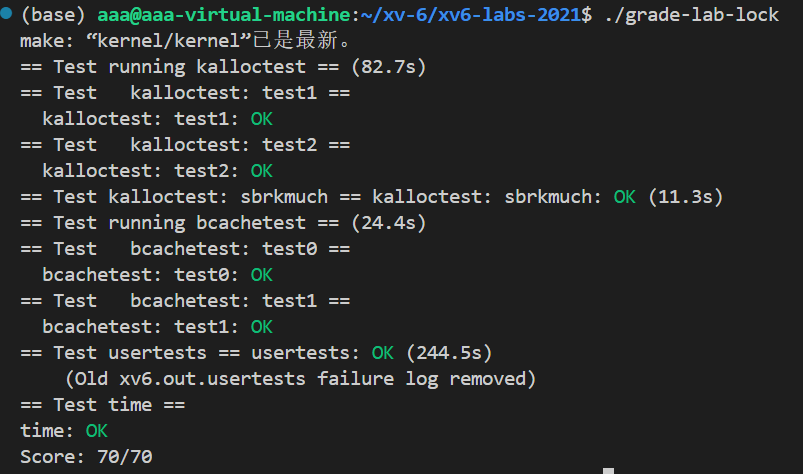
\includegraphics[width=\linewidth]{pics/lock评测结果.png}
    \caption{评测结果}
    \label{fig:lock}
\end{figure}

\subsection{实验小结}

在本次实验中,我通过对xv6系统中的内存分配器和缓冲区缓存机制进行优化,成功地提高了系统的并行性。实验的优化策略主要集中在减少锁的争用,提高系统的并行处理能力。结果表明,通过这些优化措施,系统在多核环境下的性能得到了显著提升,锁的争用情况得到了明显缓解。评测结果也验证了我的优化方案在实践中的有效性。

总的来说,本次实验通过对锁争用问题的深入分析和针对性的优化,展示了提高并行性的重要性和实现方法。未来的工作可以继续探索其他可能的优化点,例如进一步精细化锁的粒度,或是引入更高级的锁机制,以进一步提升系统的并行处理能力。








\section{Lab: File system}
\subsection{实验目的}
本实验旨在增进对操作系统的文件系统的了解。实验将会实现xv6系统对更大文件的支持,以及符号链接。目前 xv6 文件限制为 268 个块或 $268\times BSIZE$ 字节(xv6 中 BSIZE 为 1024)。这个限制是因为一个xv6 inode包含12个“直接”块号和一个“单间接”块号,这是指一个块最多可以容纳256个块号,总共$12+256=268$块。实验将更改 xv6 文件系统代码以支持每个 inode 中的“双间接”块,其中包含 256 个单间接块地址,每个块最多可包含 256 个数据块地址。结果将是一个文件最多可以包含 65803 个块,即 $256\times256+256+11$ 个块。
\subsection{实验步骤}
\subsubsection{实现Large files}
\begin{enumerate}
    \item 修改fs.h文件中的宏定义,改变文件系统块的结构。
          \begin{lstlisting}[language=c,title=修改fs.h宏定义]
    #define NDIRECT 11
    #define NINDIRECT (BSIZE / sizeof(uint))
    #define NDINDIRECT (NINDIRECT * NINDIRECT)
    #define MAXFILE (NDIRECT + NINDIRECT + NDINDIRECT)    
    \end{lstlisting}
    \item 修改fs.h中的dinode结构体,让addrs数组增加一个元素,以便储存二级索引块。
          \begin{lstlisting}[language=c,title=对dinode结构体的修改]
    struct dinode
    {
        short type;              // File type
        short major;             // Major device number (T_DEVICE only)
        short minor;             // Minor device number (T_DEVICE only)
        short nlink;             // Number of links to inode in file system
        uint size;               // Size of file (bytes)
        uint addrs[NDIRECT + 2]; // Data block addresses
    };    
    \end{lstlisting}
    \item 修改file.h中的inode结构体,修改方式同上。
          \begin{lstlisting}[language=c,title=对inode结构体的修改]
    // in-memory copy of an inode
    struct inode
    {
        uint dev;              // Device number
        uint inum;             // Inode number
        int ref;               // Reference count
        struct sleeplock lock; // protects everything below here
        int valid;             // inode has been read from disk?
    
        short type; // copy of disk inode
        short major;
        short minor;
        short nlink;
        uint size;
        uint addrs[NDIRECT + 2];
    };    
    \end{lstlisting}
    \item 修改fs.c文件中的bmap函数,增加对二级索引块的处理。
          \begin{lstlisting}[language=c,title=对bmap函数的修改]
    static uint bmap(struct inode *ip, uint bn)
    {
        uint addr, *a;
        struct buf *bp;
    
        ...
    
        // 二级索引块处理
        if (bn < NDINDIRECT)
        {
            // 检查二级间接块的起始地址是否已分配,如果未分配则分配一个新的块
            if ((addr = ip->addrs[NDIRECT + 1]) == 0)
                ip->addrs[NDIRECT + 1] = addr = balloc(ip->dev);
        
            // 读取二级间接块的数据
            bp = bread(ip->dev, addr);
            a = (uint *)bp->data;
        
            // 获取一级间接块地址,如果未分配则分配一个新的块
            if ((addr = a[bn / NINDIRECT]) == 0)
            {
                a[bn / NINDIRECT] = addr = balloc(ip->dev);
                log_write(bp);
            }
            brelse(bp);
        
            // 读取一级间接块的数据
            bp = bread(ip->dev, addr);
            a = (uint *)bp->data;
        
            // 获取最终的目标块地址,如果未分配则分配一个新的块
            if ((addr = a[bn % NINDIRECT]) == 0)
            {
                a[bn % NINDIRECT] = addr = balloc(ip->dev);
                log_write(bp);
            }
            brelse(bp);
            return addr;
        }
    
        // 如果块号超出范围,触发panic
        panic("bmap: out of range");
    }    
    \end{lstlisting}
    \item 修改fs.c文件中的itrunc函数,增加对二级索引块的处理。
          \begin{lstlisting}[language=c,title=对itrunc函数的修改]
    void itrunc(struct inode *ip)
    {
        int i, j;
        struct buf *bp, *bp2;
        uint *a, *a2;
    
        ...
    
        // 处理二级间接块
        if (ip->addrs[NDIRECT + 1])
        {
            // 读取二级间接块
            bp = bread(ip->dev, ip->addrs[NDIRECT + 1]);
            a = (uint *)bp->data;
        
            // 释放二级间接块中的每个一级间接块
            for (j = 0; j < NINDIRECT; j++)
            {
                if (a[j])
                {
                    // 读取一级间接块
                    bp2 = bread(ip->dev, a[j]);
                    a2 = (uint *)bp2->data;
            
                    // 释放一级间接块中的每个块
                    for (i = 0; i < NINDIRECT; i++)
                    {
                        if (a2[i])
                        bfree(ip->dev, a2[i]);
                    }
                    brelse(bp2);
            
                    // 释放一级间接块本身
                    bfree(ip->dev, a[j]);
                    a[j] = 0;
                }
            }
            brelse(bp);
        
            // 释放二级间接块本身
            bfree(ip->dev, ip->addrs[NDIRECT + 1]);
            ip->addrs[NDIRECT + 1] = 0;
        }
    
        // 重置inode大小并更新inode信息
        ip->size = 0;
        iupdate(ip);
    }    
    \end{lstlisting}
\end{enumerate}

\subsubsection{实现Symbolic links}
符号链接(Symbolic Link,简称symlink)是一种文件系统对象,它是一种特殊类型的文件,指向另一个文件或目录。符号链接本质上是一个包含指向目标文件或目录路径的文本文件。它允许用户在文件系统中创建一个指向另一个文件或目录的快捷方式。

\begin{enumerate}
    \item 仿照之前的方式,注册一个名为symlink的系统调用。
    \item 在stat.h中增加一个宏,表示符号链接。
          \begin{lstlisting}[language=c,title=添加表示符号链接的文件类型]
    #define T_SYMLINK 4 // Symbolic link    
    \end{lstlisting}
    \item 在fcntl.h中添加一个宏,表示不跟随符号链接的文件打开模式。
          \begin{lstlisting}[language=c,title=添加不跟随符号链接的文件打开模式的宏]
    #define O_NOFOLLOW 0x800
    \end{lstlisting}
    \item 在sysfile.c文件中实现符号链接的系统调用
          \begin{lstlisting}[language=c,title=sys\_symlink的实现]
    uint64 sys_symlink(void)
    {
        // 定义用于存储目标路径和符号链接路径的字符数组
        char target[MAXPATH], path[MAXPATH]; 
    
        // 获取符号链接指向的目标路径和符号链接路径
        // 如果获取参数失败,则返回-1
        if (argstr(0, target, MAXPATH) < 0 
        || argstr(1, path, MAXPATH) < 0)
        return -1;
    
        begin_op();       // 开始文件系统操作
        struct inode *ip; // 定义inode结构指针
    
        // 创建一个类型为符号链接的inode,路径为`path`
        // 如果创建失败,结束操作并返回-1
        if ((ip = create(path, T_SYMLINK, 0, 0)) == 0)
        {
            end_op();
            return -1;
        }
    
        // 将目标路径写入到符号链接的inode中
        // 如果写入的字节数少于MAXPATH,解锁并释放inode,然后结束操作返回-1
        if (writei(ip, 0, (uint64)target, 0, MAXPATH) < MAXPATH)
        {
            iunlockput(ip);
            end_op();
            return -1;
        }
    
        iunlockput(ip); // 解锁并释放inode
        end_op();       // 结束文件系统操作
        return 0;       // 返回0表示成功
    }    
    \end{lstlisting}
    \item 修改sysfile.c文件中的sys\_open系统调用,增加符号链接的打开方法。
          \begin{lstlisting}[language=c,title=对sys\_open函数的修改]
    uint64 sys_open(void)
    {
        char path[MAXPATH]; // 用于存储文件路径的字符数组
        int fd, omode;      // fd表示文件描述符,omode表示文件打开模式
        struct file *f;     // 文件结构指针
        struct inode *ip;   // inode结构指针
        int n;              // 临时变量,用于存储函数返回值
    
        ...
    
        // 处理符号链接,逐层解析直到达到实际文件或达到限制
        int layer = 0; // 跟踪符号链接的层数
        while (ip->type == T_SYMLINK && !(omode & O_NOFOLLOW))
        {
            layer++;                // 增加层数
            if (layer == THRESHOLD) // 如果层数达到阈值,返回错误
            {
                iunlockput(ip); // 解锁并释放inode
                end_op();       // 结束操作
                return -1;
            }
            else // 继续解析符号链接
            {
                // 读取符号链接指向的路径
                if (readi(ip, 0, (uint64)path, 0, MAXPATH) < MAXPATH)
                {
                    iunlockput(ip); // 如果读取失败,解锁并释放inode
                    end_op();       // 结束操作
                    return -1;
                }
                iunlockput(ip);   // 解锁并释放当前符号链接的inode
                ip = namei(path); // 解析符号链接指向的路径
                if (ip == 0)
                {
                    end_op(); // 如果解析失败,结束操作并返回-1
                    return -1;
                }
                ilock(ip); // 锁定解析后的inode
            }
        }
    
        ...
    
        return fd; // 返回文件描述符
    }    
    \end{lstlisting}
\end{enumerate}

\subsection{评测结果}
利用grade-lab-fs脚本评测,得到结果如图\ref{fig:fs}。
\begin{figure}[ht]
    \centering
    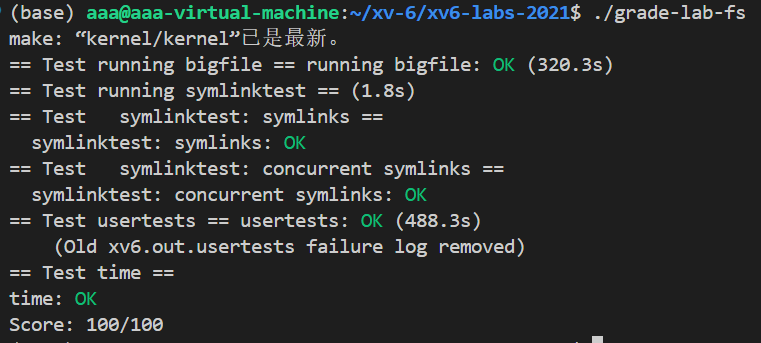
\includegraphics[width=\linewidth]{pics/fs评测结果.png}
    \caption{评测结果}
    \label{fig:fs}
\end{figure}
\subsection{实验小结}


实验完成后,我成功地为xv6文件系统增加了对大文件的支持,并实现了符号链接的功能。

在实现大文件支持时,我通过修改文件系统的块结构,引入了“双间接”块的概念,使得一个文件能够支持多达65803个块。这大幅提高了xv6系统能够处理的文件大小限制。实现过程中,我深刻理解了文件系统块管理的机制,特别是间接块的使用与管理。

符号链接的实现则为xv6文件系统增加了文件引用的灵活性。此部分实验帮助我理解了符号链接在文件系统中的作用及其实现原理。

通过对以上两个功能的实现和测试,我加深了对文件系统的理解,尤其是在文件存储结构和文件引用管理方面的知识。实验结果表明,所有功能均按预期工作,为日后深入研究和开发复杂的文件系统奠定了基础。

\section{Lab: mmap}

\subsection{实验目的}
本实验旨在熟悉进程内存地址的映射机制。mmap 和 munmap 系统调用允许 UNIX 程序对其地址空间进行详细控制。它们可用于在进程之间共享内存,将文件映射到进程地址空间,并作为用户级页面错误方案的一部分。本实验将向 xv6 添加 mmap 和 munmap,重点关注内存映射文件。

\subsection{实验步骤}

\begin{enumerate}
    \item 按照前文的方法,注册两个系统调用sys\_mmap 和sys\_munmap。
    \item 在proc.h文件中添加vma结构体,并把它添加到proc结构体中。vma 结构体表示进程的一个虚拟内存区域。虚拟内存区域用于映射进程的虚拟地址空间到实际物理内存或文件,允许进程访问所需的资源。结构体内的各个字段记录了虚拟内存区域的具体信息,包括起始地址、长度、关联的文件、保护和标志属性等。
          \begin{lstlisting}[language=c,title=vma结构体]
    // 虚拟内存区域(Virtual Memory Area, VMA)结构体
    struct vma {
        int valid;          // 标志此VMA是否有效(1表示有效,0表示无效)
        uint64 addr;        // VMA的起始地址(虚拟地址)
        int len;            // VMA的长度(以字节为单位)
        struct file *f;     // 指向与此VMA关联的文件的指针
        int prot;           // VMA的保护标志(如可读、可写、可执行)
        int flags;          // VMA的标志(如共享、私有映射)
        int fd;             // 文件描述符,用于标识与此VMA关联的文件
        int offset;         // VMA在文件中的偏移量
    };                
    \end{lstlisting}
          \begin{lstlisting}[language=c,title=对proc结构体的修改]
    #define VMASIZE 16
    struct proc
    {
      ...
      struct vma vma[VMASIZE];
    };
    \end{lstlisting}
    \item 修改trap.c文件中的usertrap 函数,添加对缺页的处理。
          \begin{lstlisting}[language=c,title=对usertrap函数的修改]
    void usertrap(void)
    {
        int which_dev = 0;
    
        ...

        else if (r_scause() == 13 || r_scause() == 15)
        {
            // 页面错误(Page Fault)
        
            // 获取发生页面错误的虚拟地址。
            uint64 va = r_stval();
        
            // 检查页面错误的地址是否在有效范围内,如果超出范围,标记进程为 killed。
            if (va >= p->sz || va > MAXVA || PGROUNDUP(va) == PGROUNDDOWN(p->trapframe->sp))
                p->killed = 1;
        
            struct vma *vma = 0;
            // 遍历进程的虚拟内存区域 (VMA),找到与页面错误地址匹配的 VMA。
            for (int i = 0; i < VMASIZE; i++)
            {
                if (p->vma[i].valid && va >= p->vma[i].addr && va < p->vma[i].addr + p->vma[i].len)
                {
                    vma = &p->vma[i];
                    break;
                }
            }
        
            if (vma)
            {
                // 将页面地址向下取整,以页大小为单位对齐。
                va = PGROUNDDOWN(va);
                uint64 offset = va - vma->addr; // 计算偏移量。
                uint64 mem = (uint64)kalloc();  // 分配一页物理内存。
                if (mem == 0)
                {
                    // 如果内存分配失败,标记进程为 killed。
                    p->killed = 1;
                }
                else
                {
                    memset((void *)mem, 0, PGSIZE); // 将分配的内存清零。
                    ilock(vma->f->ip);              // 锁定文件以防止其他进程访问。
                    readi(vma->f->ip, 0, mem, offset, PGSIZE); // 从文件中读取数据到内存中。
                    iunlock(vma->f->ip);            // 解锁文件。
            
                    // 设置页表条目的权限标志。
                    int flag = PTE_U;
                    if (vma->prot & PROT_READ)
                        flag |= PTE_R;
                    if (vma->prot & PROT_WRITE)
                        flag |= PTE_W;
                    if (vma->prot & PROT_EXEC)
                        flag |= PTE_X;
            
                    // 将虚拟地址映射到物理内存。
                    if (mappages(p->pagetable, va, PGSIZE, mem, flag) != 0)
                    {
                        // 如果映射失败,释放分配的内存并标记进程为 killed。
                        kfree((void *)mem);
                        p->killed = 1;
                    }
                }
            }
        }
        ...
    
        usertrapret(); // 从内核模式返回到用户模式,恢复进程执行。
    }    
    \end{lstlisting}
    \item 在sysfile.c文件中添加sys\_mmap和sys\_munmap系统调用的实现。
          \begin{lstlisting}[language=c,title=sys\_mmap的实现]
    uint64 sys_mmap(void)
    {
        struct file *f;       // 文件指针,指向要映射的文件
        int prot, flags, fd, offset, len;
        uint64 addr;
    
        // 从系统调用的参数中获取地址、长度、保护标志、映射标志、文件描述符和偏移量
        // 如果获取参数失败,则返回-1表示错误
        if (argaddr(0, &addr) || argint(1, &len) || argint(2, &prot) ||
            argint(3, &flags) || argfd(4, &fd, &f) || argint(5, &offset))
            return -1;
    
        // 如果文件不可写,并且请求了写权限并且映射类型是共享的,则返回-1
        if (!(f->writable) && (prot & PROT_WRITE) && flags == MAP_SHARED)
            return -1;
    
        struct proc *p = myproc();  // 获取当前进程的指针
        len = PGROUNDUP(len);       // 将长度向上对齐到页面大小
        if (p->sz > MAXVA - len)    // 如果映射超出了虚拟地址空间的最大值,则返回-1
            return -1;
    
        // 查找进程中未使用的虚拟内存区域
        for (int i = 0; i < VMASIZE; i++)
        {
            if (p->vma[i].valid == 0)  // 找到一个空闲的虚拟内存区域
            {
                // 初始化虚拟内存区域的各个属性
                p->vma[i].valid = 1;
                p->vma[i].addr = p->sz;  // 设置映射的起始地址
                p->vma[i].len = len;     // 设置映射的长度
                p->vma[i].f = f;         // 映射的文件
                p->vma[i].prot = prot;   // 保护标志
                p->vma[i].flags = flags; // 映射标志
                p->vma[i].offset = offset; // 文件偏移量
        
                filedup(f);  // 增加文件的引用计数
                p->sz += len;  // 增加进程的虚拟内存大小
        
                return p->vma[i].addr;  // 返回映射的起始地址
            }
        }
        return -1;  // 如果没有可用的虚拟内存区域,则返回-1
    }
                
    \end{lstlisting}
          \begin{lstlisting}[language=c,title=sys\_munmap的实现]
    uint64 sys_munmap(void)
    {
        uint64 addr;
        int len;
    
        // 从系统调用的参数中获取地址和长度
        // 如果获取参数失败,则返回-1表示错误
        if (argaddr(0, &addr) || argint(1, &len))
        return -1;
    
        addr = PGROUNDDOWN(addr); // 将地址向下对齐到页面大小
        len = PGROUNDUP(len);     // 将长度向上对齐到页面大小
    
        struct proc *p = myproc();  // 获取当前进程的指针
        struct vma *vma = 0;
    
        // 查找包含指定地址的虚拟内存区域
        for (int i = 0; i < VMASIZE; i++)
        {
            if (addr >= p->vma[i].addr && addr < p->vma[i].addr + p->vma[i].len)
            {
                vma = &p->vma[i];  // 找到对应的虚拟内存区域
                break;
            }
        }
    
        if (vma == 0)
            return 0;  // 如果未找到对应的虚拟内存区域,则返回0
    
        if (vma->addr == addr)  // 如果地址匹配
        {
            vma->addr += len;    // 更新虚拟内存区域的起始地址
            vma->len -= len;     // 更新虚拟内存区域的长度
        
            // 如果映射类型是共享的,将内存内容写回文件
            if (vma->flags & MAP_SHARED)
                filewrite(vma->f, addr, len);
        
            // 解除映射的内存页
            uvmunmap(p->pagetable, addr, len / PGSIZE, 1);
        
            if (vma->len == 0)  // 如果虚拟内存区域的长度为0
            {
                fileclose(vma->f);  // 关闭与该区域关联的文件
                vma->valid = 0;     // 将虚拟内存区域标记为无效
            }
        }
        return 0;  // 返回0表示成功
    }
                
    \end{lstlisting}
    \item 将vm.c文件中nvmcopy 和uvmunmap 函数的if((*pte \& PTE\_V) == 0) 条件后的panic改为continue。将 panic 改为 continue 后,当检测到无效页面时,程序不会崩溃,而是跳过这个页面,继续处理后续的页面。
    \item 在proc.c文件中修改fork函数,使之可以把父进程的内存映射也添加给子进程。
          \begin{lstlisting}[language=c,title=对fork函数的修改]
    int fork(void)
    {
        int i, pid;
        struct proc *np;         // np指向新创建的子进程结构体
        struct proc *p = myproc(); // p指向当前进程,即父进程
    
        ...
    
        // 复制父进程的虚拟内存区域(VMA)到子进程
        for (int i = 0; i < VMASIZE; i++)
        {
            if (p->vma[i].valid)  // 如果父进程的VMA有效
            {
                memmove(&(np->vma[i]), &(p->vma[i]), sizeof(p->vma[i])); // 复制VMA
                filedup(p->vma[i].f);  // 增加文件的引用计数
            }
        }
        release(&np->lock); // 释放子进程的锁
    
        return pid; // 返回子进程的PID给父进程
    }
                
    \end{lstlisting}
    \item 在proc.h文件中修改exit函数,添加接触映射的功能。
          \begin{lstlisting}[language=c,title=对exit函数的修改]
    void exit(int status)
    {
        ...
    
        // 处理进程的虚拟内存区域(VMA)
        for (int i = 0; i < VMASIZE; i++)
        {
            if (p->vma[i].valid) // 如果虚拟内存区域有效
            {
                // 如果内存映射是共享的,将内存写回文件
                if (p->vma[i].flags & MAP_SHARED)
                filewrite(p->vma[i].f, p->vma[i].addr, p->vma[i].len);
                
                // 关闭与虚拟内存区域相关联的文件
                fileclose(p->vma[i].f);
        
                // 解除映射的内存页
                uvmunmap(p->pagetable, p->vma[i].addr, p->vma[i].len / PGSIZE, 1);
        
                p->vma[i].valid = 0; // 将VMA标记为无效
            }
        }
    
        ...
    }   
                
    \end{lstlisting}
\end{enumerate}

\subsection{评测结果}
利用脚本./grade-lab-mmap评测,得到结果如图\ref{fig:mmap}。
\begin{figure}[h]
    \centering
    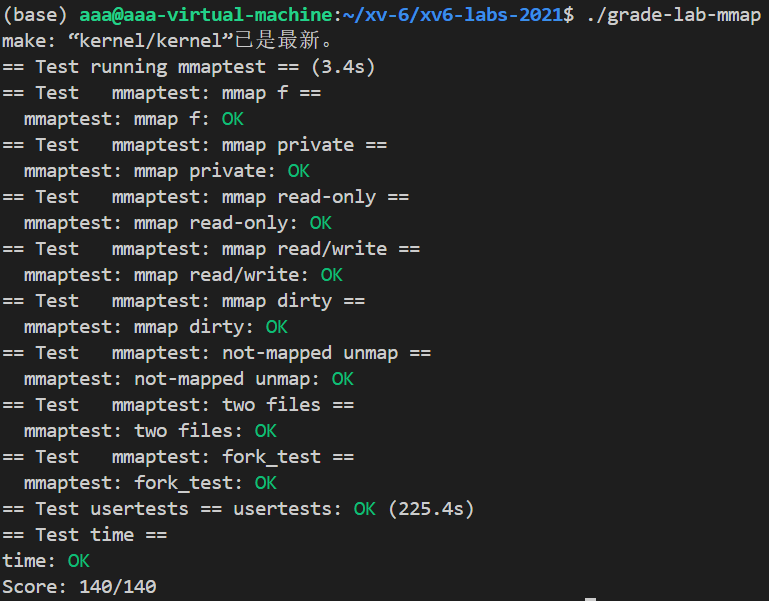
\includegraphics[width=\linewidth]{pics/mmap评测结果.png}
    \caption{mmap评测结果}
    \label{fig:mmap}
\end{figure}
\subsection{实验小结}
在本次实验中,我成功地在 xv6 操作系统中实现了 mmap 和 munmap 系统调用。通过该实验,我深入理解了内存映射的基本概念以及其在操作系统中的应用。

具体来说,我通过 sys\_mmap 系统调用实现了将文件映射到进程的虚拟内存地址空间的功能,使得进程可以直接通过内存访问文件内容,而无需频繁的文件 I/O 操作。这不仅提升了文件访问的效率,还为进程间共享内存提供了基础。

总体而言,本实验使我掌握了内存映射的核心机制,并在 xv6 中实现了这一功能,进一步加深了对操作系统内存管理的理解。这些知识不仅对理解现代操作系统的内存管理至关重要,也为后续的系统开发和优化提供了实践经验。


\end{document}
